\documentclass[12pt,a4paper]{article}

\usepackage[utf8]{inputenc}
\usepackage[T1]{fontenc}
\usepackage[spanish,provide=*]{babel}
\usepackage{geometry}
\geometry{margin=1in}
\usepackage{hyperref}
\hypersetup{
    colorlinks=true,
    linkcolor=blue,
    filecolor=magenta,
    urlcolor=cyan,
}
\usepackage{listings}
\lstset{
    language=bash,
    basicstyle=\ttfamily\footnotesize,
    breaklines=true,
    captionpos=b,
    numbers=left,
    numberstyle=\tiny,
    frame=single,
    backgroundcolor=\color{gray!10},
    extendedchars=true,
    inputencoding=utf8,
    literate={á}{{\'a}}1 {é}{{\'e}}1 {í}{{\'i}}1 {ó}{{\'o}}1 {ú}{{\'u}}1 {ñ}{{\~n}}1 {Á}{{\'A}}1 {É}{{\'E}}1 {Í}{{\'I}}1 {Ó}{{\'O}}1 {Ú}{{\'U}}1 {Ñ}{{\~N}}1
}
\usepackage{graphicx}
\usepackage{tabularx}
\usepackage{svg}
\usepackage{fancyhdr}
\pagestyle{fancy}
\fancyhf{}
\fancyhead[L]{\leftmark}
\fancyhead[R]{\thepage}

\usepackage{xcolor}
\definecolor{codebg}{rgb}{0.95,0.95,0.95}

\setlength{\parskip}{0.5\baselineskip}

\let\oldsection\section
\renewcommand{\section}{\newpage\oldsection}

\title{Clúster Kind con Soporte para GPU}
\author{Documentación Completa}
\date{\today}

\begin{document}

\maketitle

\begin{abstract}
Esta documentación proporciona una guía completa y profesional para configurar un clúster Kubernetes local utilizando Kind con soporte avanzado para GPUs NVIDIA. Incluye instalación automatizada, scripts, ejemplos prácticos y soluciones a problemas comunes, facilitando el aprendizaje y desarrollo en entornos de inteligencia artificial y computación intensiva. Dirigido a desarrolladores, investigadores y estudiantes, el documento democratiza el acceso a tecnologías avanzadas sin depender de recursos costosos en la nube.
\end{abstract}

\newpage
\section{Prólogo}

En un mundo donde la computación en la nube y la inteligencia artificial avanzan a pasos agigantados, la necesidad de entornos de desarrollo locales eficientes y accesibles se vuelve cada vez más crítica. Esta documentación surge de la experiencia práctica en el despliegue de clústeres de Kubernetes utilizando Kind, con un enfoque especial en la integración de GPU para aplicaciones de alto rendimiento.

Como Líder de IA y Arquitecto de Soluciones, he observado cómo las barreras técnicas pueden frenar la innovación. Esta guía no solo proporciona instrucciones técnicas detalladas, sino que también busca democratizar el acceso a tecnologías avanzadas, permitiendo a desarrolladores, investigadores y estudiantes experimentar con Kubernetes y GPU sin depender de recursos en la nube costosos o complejos.

El objetivo es empoderar a la comunidad tecnológica, facilitando el aprendizaje y la experimentación. Cada sección ha sido diseñada pensando en la practicidad, con ejemplos reales, soluciones a problemas comunes y herramientas automatizadas que reducen la curva de aprendizaje.

Que esta documentación sea un puente entre la teoría y la práctica, inspirando nuevas ideas y proyectos en el fascinante mundo de la orquestación de contenedores y la computación acelerada.

William R. (wisrovi-rodriguez)

\newpage
\tableofcontents

\newpage
\listoffigures

\newpage
\listoftables
\newpage
\lstlistoflistings
\newpage

\section{Acerca del Autor}

\begin{minipage}{0.3\textwidth}
    
\includegraphics[width=\linewidth]{resources/william-perfil.jpeg}
\end{minipage}
\hfill
\begin{minipage}{0.65\textwidth}
    \textbf{William R. (wisrovi-rodriguez)} \\
    Líder de IA y Arquitecto de Soluciones en eCaptureDtech. \\
    Ubicación: Badajoz, Extremadura, España. \\
    \\
    Como Líder de IA y Arquitecto de Soluciones en eCaptureDtech, mi misión es forjar el futuro de la tecnología mediante la integración de inteligencia artificial avanzada en soluciones empresariales. Con una sólida formación en ingeniería y una pasión por la innovación, he dedicado mi carrera a explorar las fronteras de la IA, desde el desarrollo de algoritmos de aprendizaje automático hasta la implementación de sistemas de IA generativa. \\
    \\
    Mi experiencia abarca desde la investigación académica hasta el liderazgo en proyectos tecnológicos, colaborando con equipos multidisciplinarios para resolver desafíos complejos. Soy un apasionado de la educación y el compartir conocimiento, contribuyendo activamente a la comunidad tecnológica a través de publicaciones, conferencias y proyectos open-source. \\
    \\
    En mi rol actual, me enfoco en diseñar arquitecturas escalables que aprovechen el poder de la IA para transformar industrias, siempre con un enfoque ético y sostenible. \\
    \\
    \textbf{Contacto:} \\
    LinkedIn: \url{https://es.linkedin.com/in/wisrovi-rodriguez} \\
    GitHub: \url{https://github.com/wisrovi}
\end{minipage}

\newpage

\newpage
\section{Introducción}

Esta documentación aborda la configuración de un clúster Kubernetes local usando Kind con soporte para GPUs NVIDIA, facilitando el desarrollo y aprendizaje en entornos de IA. Siguiendo la visión del prólogo de democratizar tecnologías avanzadas, el documento proporciona una guía paso a paso, desde prerrequisitos hasta ejemplos avanzados.

\subsection{¿Qué es Kind?}

\begin{figure}[h]
\centering
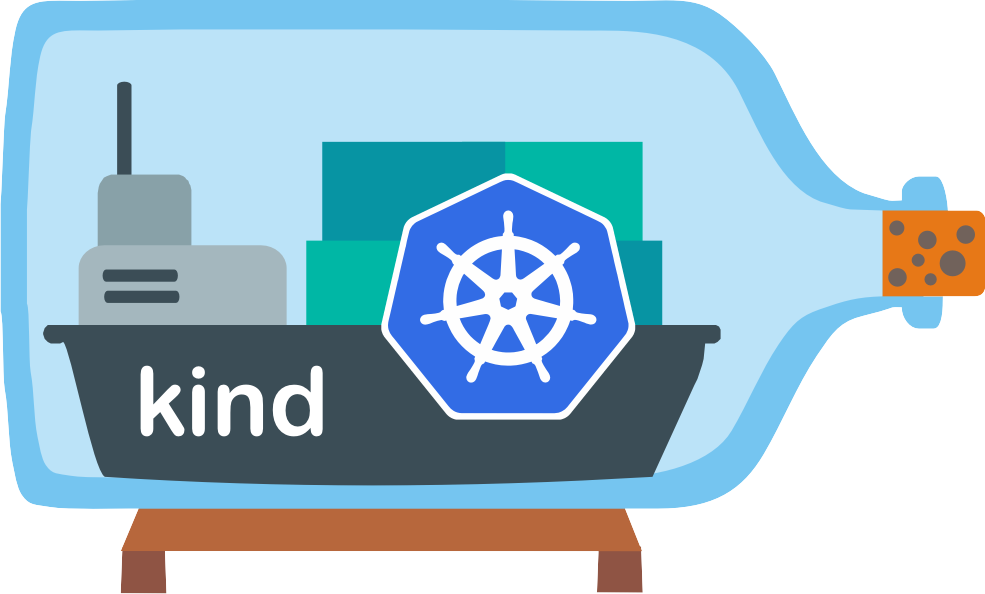
\includegraphics[width=0.5\textwidth]{resources/kind-logo.png}
\caption{Logo de Kind}
\label{fig:kind-logo}
\end{figure}

Kind (Kubernetes in Docker) es una herramienta que ejecuta clústeres Kubernetes locales usando contenedores Docker. Ideal para desarrollo, pruebas y aprendizaje, permite experimentar con configuraciones avanzadas sin costos de nube.

\subsection{Beneficios de Usar Kind con GPUs}

Integra GPUs para procesamiento local de IA, desarrollo eficiente, ahorro de costos y reproducibilidad en entornos locales.

\subsection{Glosario}

\begin{description}
    \item[ArgoCD] Herramienta de GitOps para Kubernetes que automatiza el despliegue y gestión de aplicaciones.
    \item[Cluster] Conjunto de nodos interconectados que trabajan juntos para ejecutar aplicaciones distribuidas.
    \item[Docker] Plataforma de contenedorización que permite empaquetar, distribuir y ejecutar aplicaciones en entornos aislados llamados contenedores.
    \item[GPU] Unidad de Procesamiento Gráfico, utilizada para acelerar tareas de computación intensiva como el procesamiento de imágenes y aprendizaje automático.
    \item[k9s] Interfaz de usuario basada en terminal para gestionar clústeres de Kubernetes de manera eficiente.
    \item[Kind] Herramienta para ejecutar clústeres de Kubernetes locales utilizando contenedores Docker como nodos.
    \item[Kubernetes] Plataforma de orquestación de contenedores de código abierto para automatizar el despliegue, escalado y gestión de aplicaciones en contenedores.
    \item[Node] Máquina física o virtual en un clúster de Kubernetes que ejecuta pods y es gestionada por el plano de control.
    \item[NVIDIA] Empresa líder en tecnología de GPUs y computación paralela, proveedora de drivers y toolkits para GPUs.
    \item[Pod] La unidad más pequeña y básica en Kubernetes, que representa un conjunto de contenedores que comparten recursos y red.
\end{description}

\newpage
\section{Instalación de Dependencias}

Antes de comenzar con Kind, es necesario instalar las herramientas básicas como Docker, NVIDIA Container Toolkit y Docker Compose.

\subsection{Instalar Docker}



Docker es una plataforma de contenedorización de código abierto que permite empaquetar, distribuir y ejecutar aplicaciones en entornos aislados llamados contenedores. Es esencial para Kind, ya que Kind utiliza contenedores Docker para simular nodos de Kubernetes, proporcionando un entorno ligero y reproducible.

\begin{figure}[h]
\centering
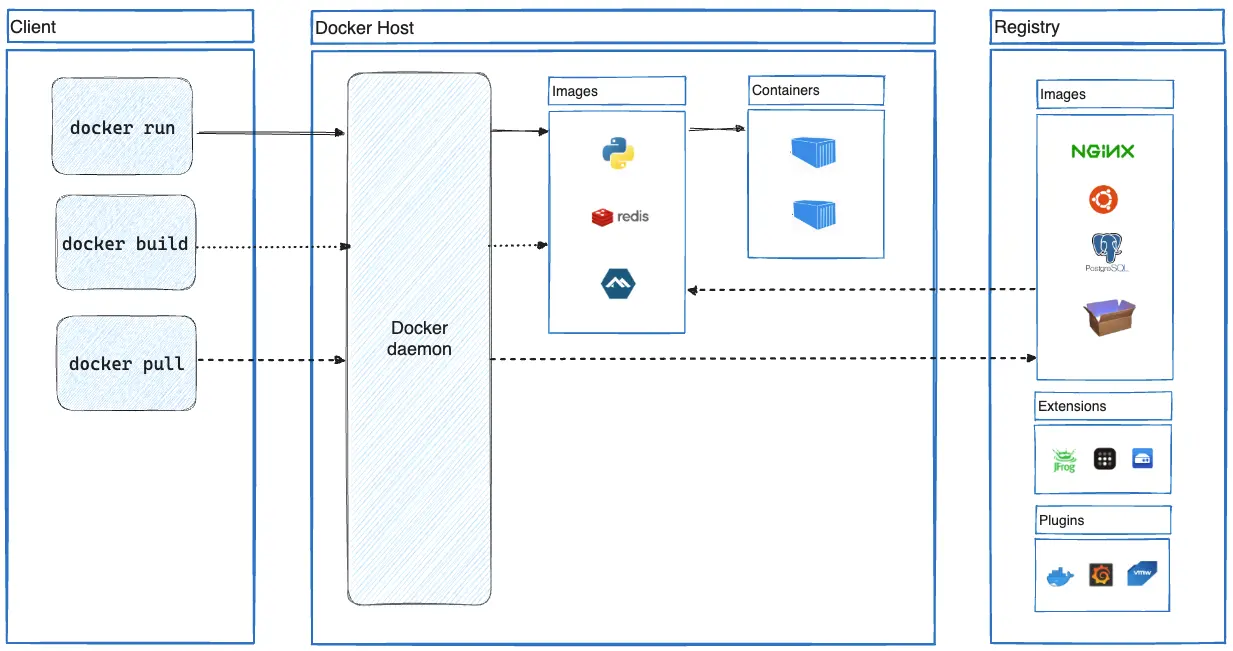
\includegraphics[width=\textwidth]{resources/docker-architecture.png}
\caption{Arquitectura de Docker}
\label{fig:docker-architecture}
\end{figure}

Basado en: \url{https://docs.docker.com/engine/install/ubuntu/}

\begin{lstlisting}[language=bash,caption={Instalación de Docker en Ubuntu}]
# Actualizar el sistema
sudo apt update

# Instalar Docker
sudo apt install -y docker.io

# Iniciar y habilitar Docker
sudo systemctl start docker
sudo systemctl enable docker

# Agregar usuario al grupo docker (opcional)
sudo usermod -aG docker $USER

# Verificar instalacion
docker --version
\end{lstlisting}

Salida esperada:

\begin{figure}[h]
\centering
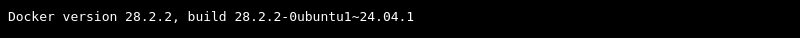
\includegraphics[width=\textwidth]{resources/results/docker_version.png}
\caption{Salida del comando docker --version}
\end{figure}

\subsection{Instalar NVIDIA Container Toolkit}

\begin{figure}[h]
\begin{center}

\includegraphics[width=0.3\textwidth]{resources/nvidia-logo.png}
\caption{Logo de NVIDIA}
\label{fig:nvidia-logo}
\end{center}
\end{figure}

El NVIDIA Container Toolkit permite que los contenedores Docker accedan a GPUs NVIDIA, habilitando el paso a través de dispositivos para aplicaciones que requieren aceleración GPU. Es crucial para ejecutar cargas de trabajo de IA o computación intensiva en contenedores.



Basado en: \url{https://docs.nvidia.com/datacenter/cloud-native/container-toolkit/latest/install-guide.html}

\begin{lstlisting}[language=bash,caption={Instalación del NVIDIA Container Toolkit}]
# Instalar prerrequisitos
sudo apt-get update && sudo apt-get install -y --no-install-recommends \
   curl \
   gnupg2

# Configurar repositorio
curl -fsSL https://nvidia.github.io/libnvidia-container/gpgkey | sudo gpg --dearmor -o /usr/share/keyrings/nvidia-container-toolkit-keyring.gpg \
  && curl -s -L https://nvidia.github.io/libnvidia-container/stable/deb/nvidia-container-toolkit.list | \
    sed 's#deb https://#deb \[signed-by=/usr/share/keyrings/nvidia-container-toolkit-keyring.gpg\] https://#g' | \
    sudo tee /etc/apt/sources.list.d/nvidia-container-toolkit.list

# Actualizar paquetes
sudo apt-get update

# Instalar NVIDIA Container Toolkit
export NVIDIA_CONTAINER_TOOLKIT_VERSION=1.18.0-1
sudo apt-get install -y \
    nvidia-container-toolkit=${NVIDIA_CONTAINER_TOOLKIT_VERSION} \
    nvidia-container-toolkit-base=${NVIDIA_CONTAINER_TOOLKIT_VERSION} \
    libnvidia-container-tools=${NVIDIA_CONTAINER_TOOLKIT_VERSION} \
    libnvidia-container1=${NVIDIA_CONTAINER_TOOLKIT_VERSION}

# Configurar runtime para Docker
sudo nvidia-ctk runtime configure --runtime=docker
sudo systemctl restart docker

# Verificar
docker run --rm --gpus all nvidia/cuda:11.0-base nvidia-smi
\end{lstlisting}

Salida esperada (ejemplo):

\begin{lstlisting}[caption={Salida del comando nvidia-smi}]
Thu Nov 13 08:58:20 2025
+-----------------------------------------------------------------------------------------+
| NVIDIA-SMI 575.64.03              Driver Version: 575.64.03      CUDA Version: 12.9     |
|-----------------------------------------+------------------------+----------------------+
| GPU  Name                 Persistence-M | Bus-Id          Disp.A | Volatile Uncorr. ECC |
| Fan  Temp   Perf          Pwr:Usage/Cap |           Memory-Usage | GPU-Util  Compute M. |
|                                         |                        |               MIG M. |
|=========================================+========================+======================|
|   0  NVIDIA GeForce RTX 3060        Off |   00000000:01:00.0  On |                  N/A |
|  0%   39C    P8             14W /  170W |    1861MiB /  12288MiB |     30%      Default |
|                                         |                        |                  N/A |
+-----------------------------------------+------------------------+----------------------+

+-----------------------------------------------------------------------------------------+
| Processes:                                                                              |
|  GPU   GI   CI              PID   Type   Process name                        GPU Memory |
|        ID   ID                                                               Usage      |
|=========================================================================================|
|    0   N/A  N/A            5157      G   /usr/lib/xorg/Xorg                      357MiB |
...
\end{lstlisting}

\subsection{Instalar Docker Compose}

\begin{figure}[h]
\begin{center}

\includegraphics[width=0.3\textwidth]{resources/docker-compose-logo-converted.png}
\caption{Logo de Docker Compose}
\label{fig:docker-compose-logo}
\end{center}
\end{figure}

Docker Compose es una herramienta para definir y ejecutar aplicaciones Docker multi-contenedor utilizando archivos YAML. Facilita la gestión de entornos complejos con múltiples servicios interconectados.

Basado en: \url{https://docs.docker.com/compose/install/}

\begin{lstlisting}[language=bash,caption={Instalación de Docker Compose}]
# Descargar Docker Compose
sudo curl -L "https://github.com/docker/compose/releases/download/v2.24.0/docker-compose-$(uname -s)-$(uname -m)" -o /usr/local/bin/docker-compose

# Hacer ejecutable
sudo chmod +x /usr/local/bin/docker-compose

# Verificar
docker-compose --version
\end{lstlisting}



\subsection{Instalar kubectl}

\begin{figure}[h]
\begin{center}
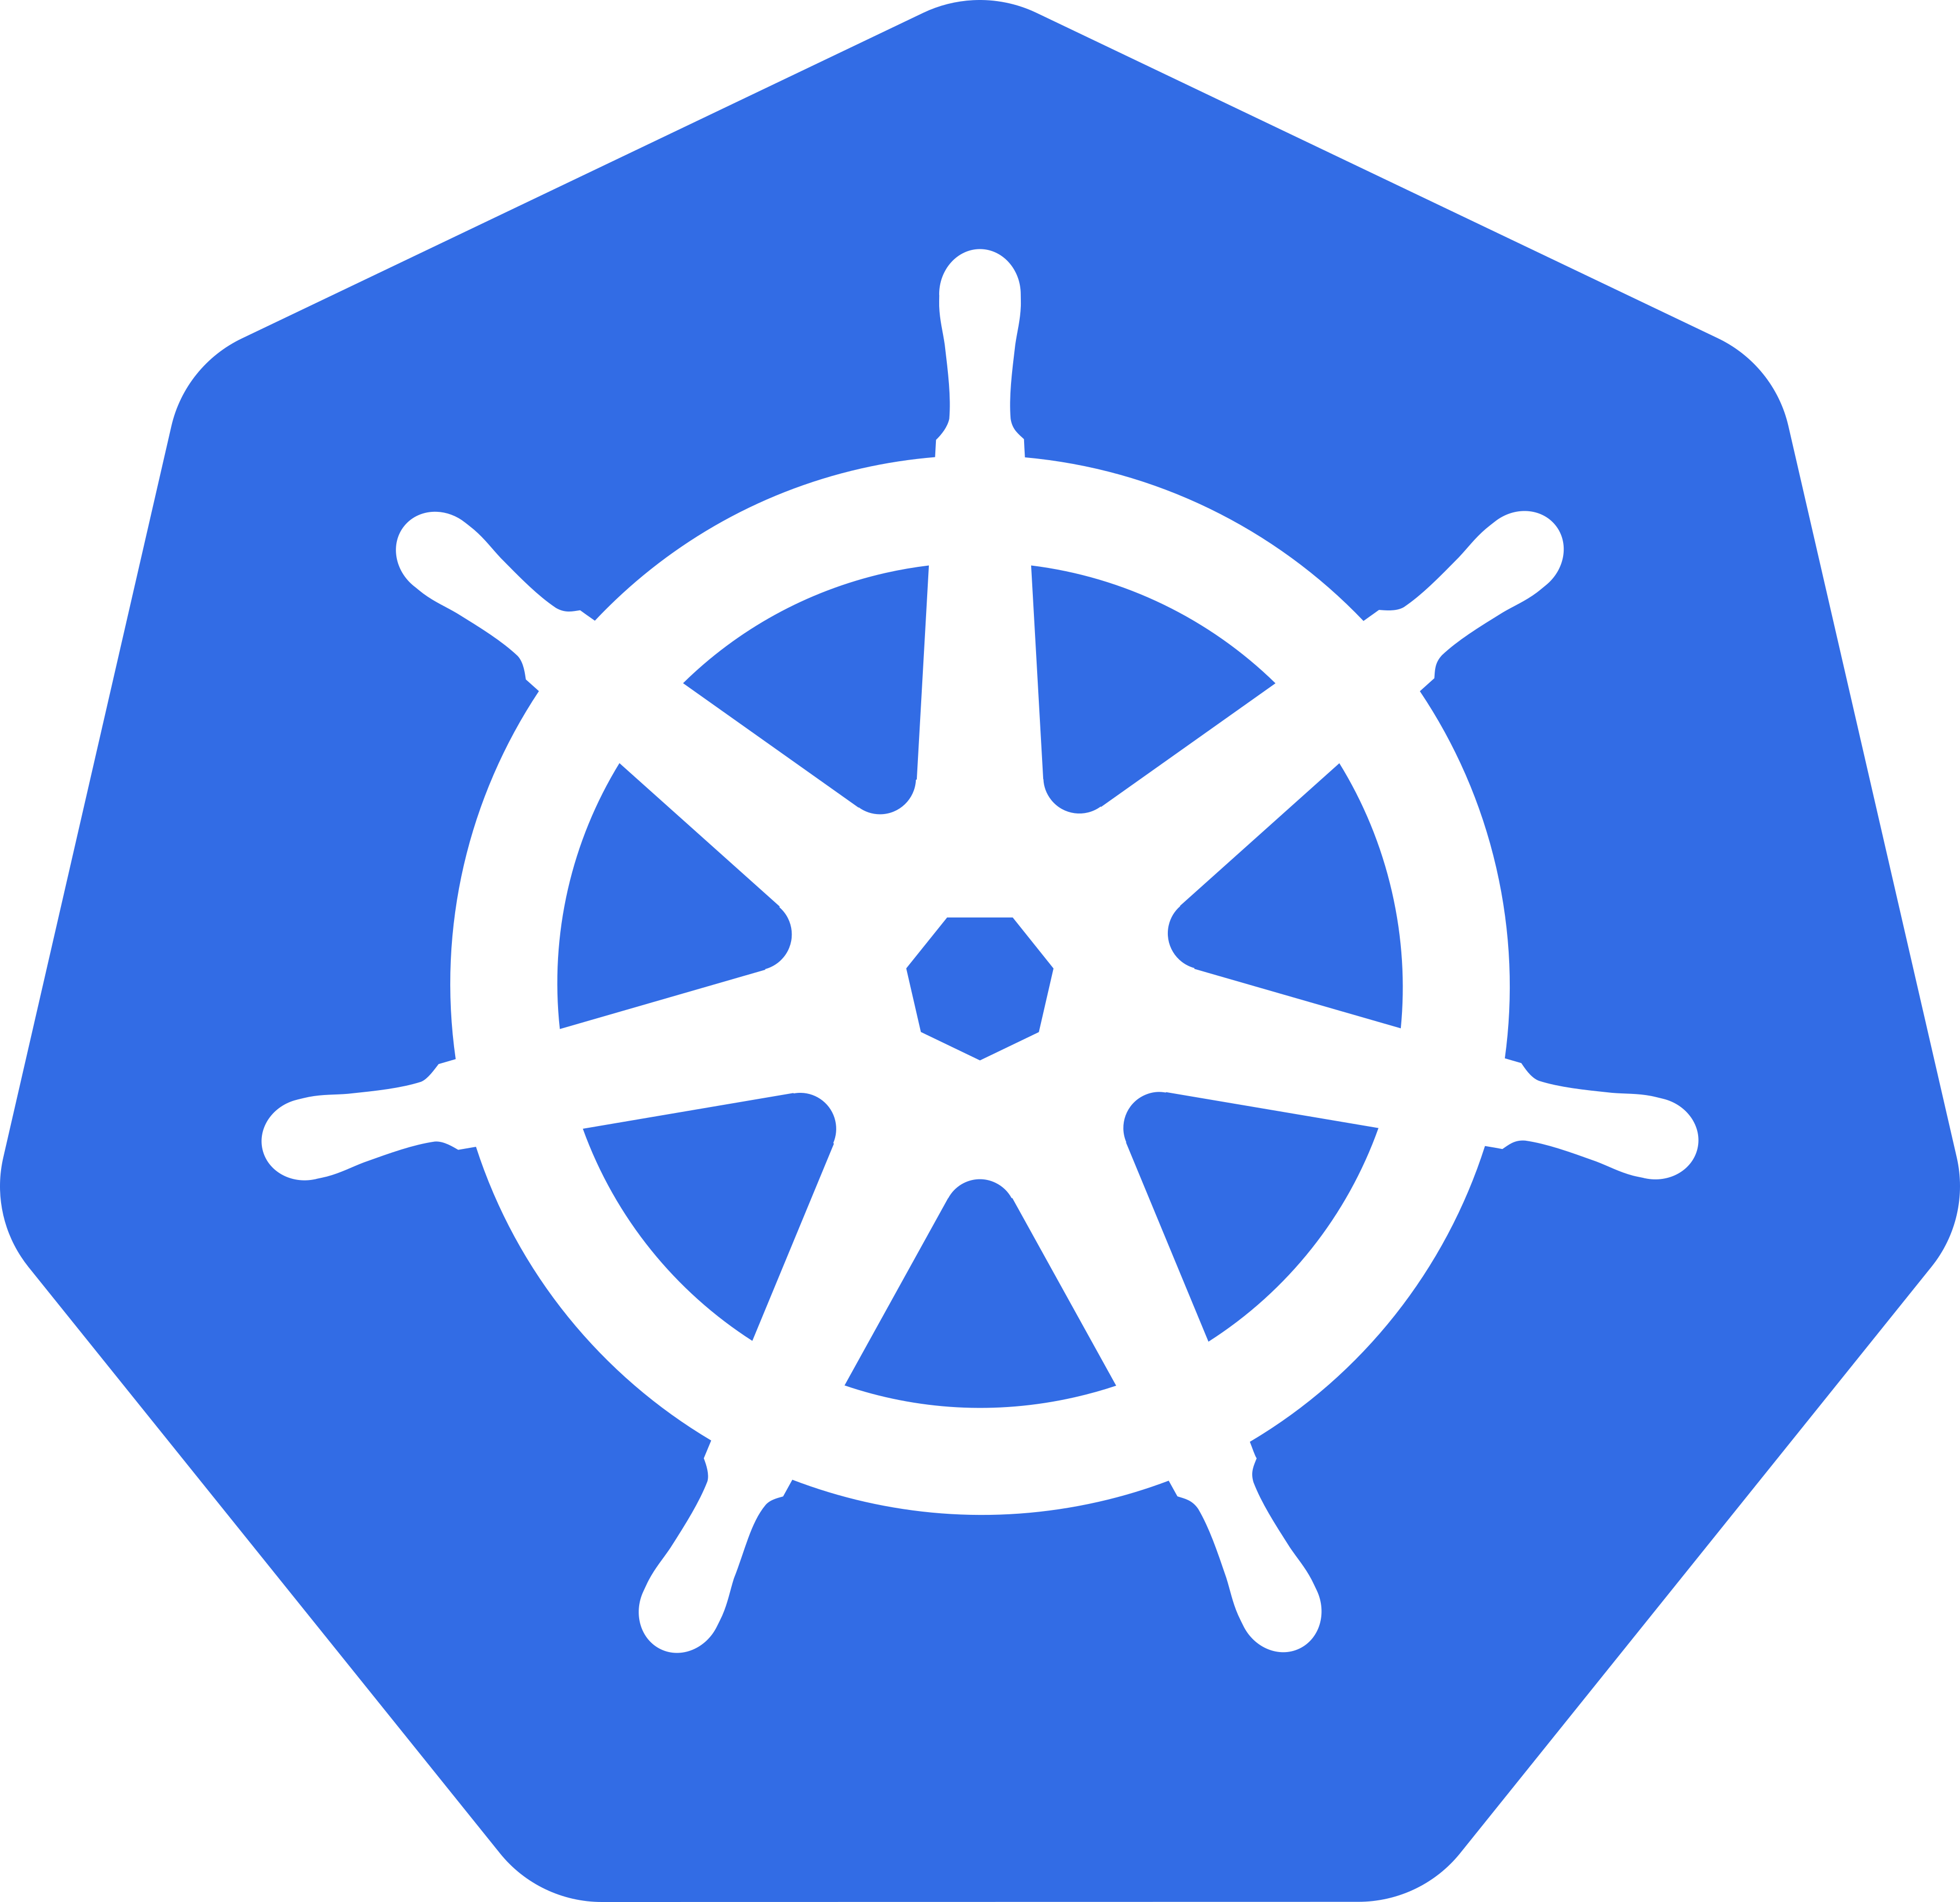
\includegraphics[width=0.3\textwidth]{resources/kubectl-logo-converted.png}
\caption{Logo de kubectl}
\label{fig:kubectl-logo}
\end{center}
\end{figure}

kubectl es la herramienta de línea de comandos oficial para interactuar con clústeres de Kubernetes, permitiendo desplegar aplicaciones, inspeccionar recursos y gestionar el clúster.

Basado en: \url{https://kubernetes.io/docs/tasks/tools/install-kubectl-linux/}

\begin{lstlisting}[language=bash,caption={Instalación de kubectl}]
# Descargar la ultima version
curl -LO "https://dl.k8s.io/release/$(curl -L -s https://dl.k8s.io/release/stable.txt)/bin/linux/amd64/kubectl"

# Hacer ejecutable
chmod +x kubectl

# Mover a PATH
sudo mv kubectl /usr/local/bin/

# Verificar
kubectl version --client
\end{lstlisting}

\begin{figure}[h]
\centering
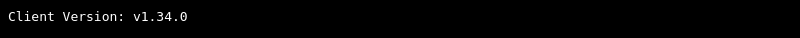
\includegraphics[width=\textwidth]{resources/results/kubectl_version.png}
\caption{Salida del comando kubectl version --client}
\end{figure}

\begin{figure}[h]
\centering
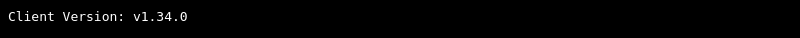
\includegraphics[width=\textwidth]{resources/results/kubectl_version.png}
\caption{Salida del comando kubectl version --client}
\end{figure}

\subsection{Instalar containerd}

\begin{figure}[h]
\begin{center}

\includegraphics[width=0.3\textwidth]{resources/containerd-logo-converted.png}
\caption{Logo de containerd}
\label{fig:containerd-logo}
\end{center}
\end{figure}

containerd es un runtime de contenedores de alto rendimiento, utilizado por Kubernetes como CRI (Container Runtime Interface) para gestionar el ciclo de vida de contenedores.

Basado en: \url{https://containerd.io/docs/getting-started/}

\begin{lstlisting}[language=bash,caption={Instalación de containerd}]
# Instalar dependencias
sudo apt-get update
sudo apt-get install -y ca-certificates curl gnupg lsb-release

# Agregar clave GPG
sudo mkdir -p /etc/apt/keyrings
curl -fsSL https://download.docker.com/linux/ubuntu/gpg | sudo gpg --dearmor -o /etc/apt/keyrings/docker.gpg

# Agregar repositorio
echo "deb [arch=$(dpkg --print-architecture) signed-by=/etc/apt/keyrings/docker.gpg] https://download.docker.com/linux/ubuntu $(lsb_release -cs) stable" | sudo tee /etc/apt/sources.list.d/docker.list > /dev/null

# Instalar containerd
sudo apt-get update
sudo apt-get install -y containerd.io

# Verificar
containerd --version
\end{lstlisting}

\begin{figure}[h]
\centering
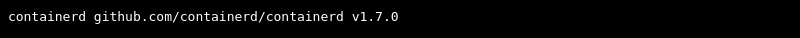
\includegraphics[width=\textwidth]{resources/results/containerd_version.png}
\caption{Salida del comando containerd --version}
\end{figure}

\subsection{Instalar etcd}

\begin{figure}[h]
\begin{center}

\includegraphics[width=0.3\textwidth]{resources/etcd-logo-horizontal.png}
\caption{Logo de etcd}
\label{fig:etcd-logo}
\end{center}
\end{figure}

etcd es un almacén de clave-valor distribuido y consistente, utilizado por Kubernetes para almacenar datos de configuración y estado del clúster.

Basado en: \url{https://etcd.io/docs/v3.5/install/}

\begin{lstlisting}[language=bash,caption={Instalación de etcd}]
# Descargar etcd
ETCD_VER=v3.5.9
DOWNLOAD_URL=https://github.com/etcd-io/etcd/releases/download
curl -L ${DOWNLOAD_URL}/${ETCD_VER}/etcd-${ETCD_VER}-linux-amd64.tar.gz -o /tmp/etcd-${ETCD_VER}-linux-amd64.tar.gz

# Extraer
tar xzvf /tmp/etcd-${ETCD_VER}-linux-amd64.tar.gz -C /tmp/
sudo mv /tmp/etcd-${ETCD_VER}-linux-amd64/etcd* /usr/local/bin/

# Verificar
etcd --version
\end{lstlisting}

\begin{figure}[h]
\centering
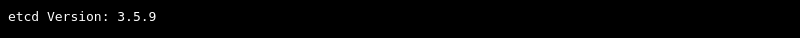
\includegraphics[width=\textwidth]{resources/results/etcd_version.png}
\caption{Salida del comando etcd --version}
\end{figure}

\subsection{Instalar kubelet}

kubelet es el agente principal que se ejecuta en cada nodo de Kubernetes, responsable de gestionar los contenedores y reportar el estado al plano de control.

Basado en: \url{https://kubernetes.io/docs/setup/production-environment/tools/kubeadm/install-kubeadm/}

\begin{lstlisting}[language=bash,caption={Instalación de kubelet}]
# Descargar kubelet
KUBE_VER=$(curl -L -s https://dl.k8s.io/release/stable.txt)
curl -LO "https://dl.k8s.io/release/${KUBE_VER}/bin/linux/amd64/kubelet"

# Hacer ejecutable
chmod +x kubelet

# Mover a PATH
sudo mv kubelet /usr/local/bin/

# Verificar
kubelet --version
\end{lstlisting}

\begin{figure}[h]
\centering
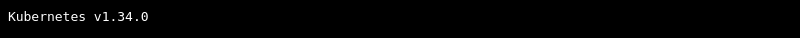
\includegraphics[width=\textwidth]{resources/results/kubelet_version.png}
\caption{Salida del comando kubelet --version}
\end{figure}

\newpage
\tableofcontents
\newpage
\section{Objetivos del Proyecto}

Este proyecto tiene como objetivos principales proporcionar una configuración completa y profesional para crear un clúster de Kubernetes utilizando Kind con soporte para GPUs NVIDIA. Incluye scripts automatizados, documentación detallada y ejemplos prácticos para facilitar la implementación y el uso.

Los objetivos específicos se dividen en las siguientes categorías:

\begin{itemize}
    \item \textbf{Configuración Completa:} Proporcionar una guía paso a paso para instalar y configurar un clúster Kind con soporte GPU.
    \item \textbf{Automatización:} Incluir scripts automatizados para simplificar la instalación y verificación.
    \item \textbf{Documentación Profesional:} Ofrecer documentación detallada con ejemplos y soluciones a problemas comunes.
    \item \textbf{Soporte para GPUs:} Habilitar el uso de GPUs NVIDIA en contenedores Kubernetes para aplicaciones de IA y computación intensiva.
    \item \textbf{Facilitación del Aprendizaje:} Democratizar el acceso a tecnologías avanzadas para desarrolladores, investigadores y estudiantes.
\end{itemize}

Para lograr estos objetivos, el proyecto se estructura en fases claras: desde la verificación de requisitos hasta la implementación, verificación y uso práctico del clúster.

\newpage
\section{Requisitos del Sistema}

Antes de comenzar la implementación, es esencial verificar que su sistema cumpla con los requisitos mínimos. Esta sección detalla los prerrequisitos en hardware, software, red y permisos necesarios para un funcionamiento óptimo del clúster Kind con soporte GPU.

\subsection{Hardware}

\begin{table}[h]
\centering
\caption{Requisitos de Hardware}
\label{tab:requisitos-hardware}
\begin{tabular}{|l|p{10cm}|}
\hline
\textbf{Requisito} & \textbf{Descripción} \\
\hline
GPU NVIDIA & Una GPU NVIDIA compatible, como RTX 3060, necesaria para ejecutar cargas de trabajo con aceleración GPU en contenedores. Sin una GPU compatible, no se pueden aprovechar las capacidades de procesamiento paralelo para aplicaciones de IA o computación intensiva. \\
\hline
RAM & Al menos 8 GB de RAM para ejecutar el clúster Kind con varios nodos, incluyendo el plano de control y trabajadores. La RAM insuficiente puede causar fallos en la creación del clúster o lentitud en las operaciones. \\
\hline
CPU & Mínimo 4 núcleos de CPU para un rendimiento adecuado del clúster, permitiendo la ejecución simultánea de componentes de Kubernetes y aplicaciones. Menos núcleos pueden resultar en tiempos de respuesta lentos. \\
\hline
\end{tabular}
\end{table}

\subsection{Software}

\begin{table}[h]
\centering
\caption{Requisitos de Software}
\label{tab:requisitos-software}
\begin{tabular}{|l|p{10cm}|}
\hline
\textbf{Requisito} & \textbf{Descripción} \\
\hline
Docker & Versión 20.10+ requerida para ejecutar Kind y los contenedores del clúster. Docker actúa como el motor de contenedorización subyacente que Kind utiliza para crear nodos simulados. \\
\hline
Drivers NVIDIA & Versión 575.64.03+ con CUDA 12.9 para acceso a GPU. Estos drivers permiten la comunicación entre el sistema operativo y la GPU, esencial para aplicaciones que requieren CUDA. \\
\hline
Kernel Linux & Versión 5.4+ para soporte de paso a través de dispositivos GPU. Un kernel más antiguo puede no admitir el montaje directo de dispositivos GPU en contenedores. \\
\hline
curl/wget & Herramientas de línea de comandos para descargas de scripts, imágenes y paquetes desde internet, necesarias durante la instalación. \\
\hline
\end{tabular}
\end{table}

\subsection{Red}

\begin{table}[h]
\centering
\caption{Requisitos de Red}
\label{tab:requisitos-red}
\begin{tabular}{|l|p{10cm}|}
\hline
\textbf{Requisito} & \textbf{Descripción} \\
\hline
Puertos & Puertos 12741-12761 disponibles para exposición de servicios del clúster. Estos puertos se utilizan para acceder a aplicaciones desplegadas en el clúster desde el host local. \\
\hline
Internet & Acceso a internet para descarga de imágenes de contenedores y componentes de Kubernetes. Sin conexión, se requieren imágenes pre-descargadas o un registro local. \\
\hline
\end{tabular}
\end{table}

\subsection{Permisos}

\begin{table}[h]
\centering
\caption{Requisitos de Permisos}
\label{tab:requisitos-permisos}
\begin{tabular}{|l|p{10cm}|}
\hline
\textbf{Requisito} & \textbf{Descripción} \\
\hline
Sudo & Acceso sudo para instalación de Kind y herramientas del sistema. Permite ejecutar comandos con privilegios elevados necesarios para instalar paquetes y modificar configuraciones del sistema. \\
\hline
Grupo Docker & Membresía en el grupo Docker o permisos sudo para ejecutar comandos Docker. Sin esto, los comandos Docker fallarán debido a permisos insuficientes. \\
\hline
\end{tabular}
\end{table}

\subsection{Verificación de Prerrequisitos}

Ejecute \texttt{./scripts/validate.sh}\footnote{En caso de no encontrar el script, puede crearlo usando el Anexo 2.} para verificar automáticamente que todos los requisitos del sistema estén cumplidos. Este script realiza comprobaciones de hardware, software y permisos, proporcionando un informe detallado de cualquier problema potencial.

\newpage
\section{Instalación de Herramientas}

Esta sección describe los pasos para instalar las herramientas necesarias.

**Nota:** Para una instalación automatizada completa, incluyendo todas las dependencias y pruebas, utilice el script \texttt{mega\_setup.sh} (requiere sudo). Consulte el Anexo 8 para más detalles.

\subsection{Instalar Kind}

Kind es la herramienta principal para crear y gestionar clústeres de Kubernetes locales usando Docker. Simplifica el desarrollo y pruebas al proporcionar un entorno reproducible.

Basado en: \url{https://kind.sigs.k8s.io/docs/user/quick-start/}

\begin{figure}[h]
\centering
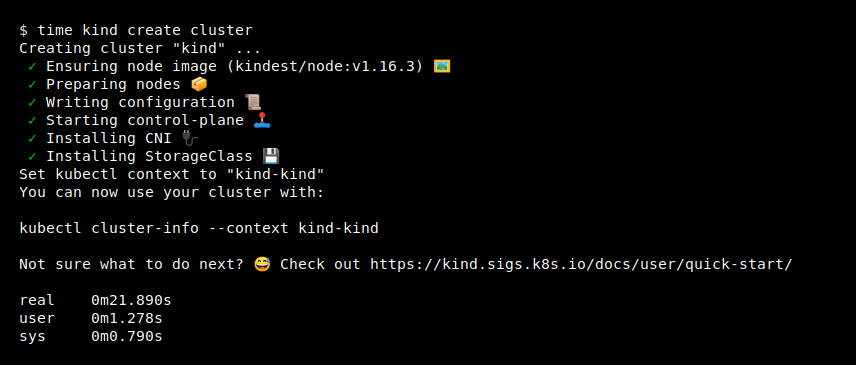
\includegraphics[width=\textwidth]{resources/kind-quick-start.png}
\caption{Guía de inicio rápido de Kind}
\label{fig:kind-quick-start}
\end{figure}

\begin{lstlisting}
curl -Lo ./kind https://kind.sigs.k8s.io/dl/v0.30.0/kind-linux-amd64
chmod +x ./kind
sudo mv ./kind /usr/local/bin/kind
kind --version
\end{lstlisting}

\begin{figure}[h]
\centering
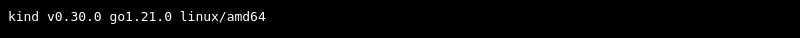
\includegraphics[width=\textwidth]{resources/results/kind_version.png}
\caption{Salida del comando kind --version}
\end{figure}

\newpage
\section{Arquitectura del Clúster}

\begin{figure}[h]
\centering
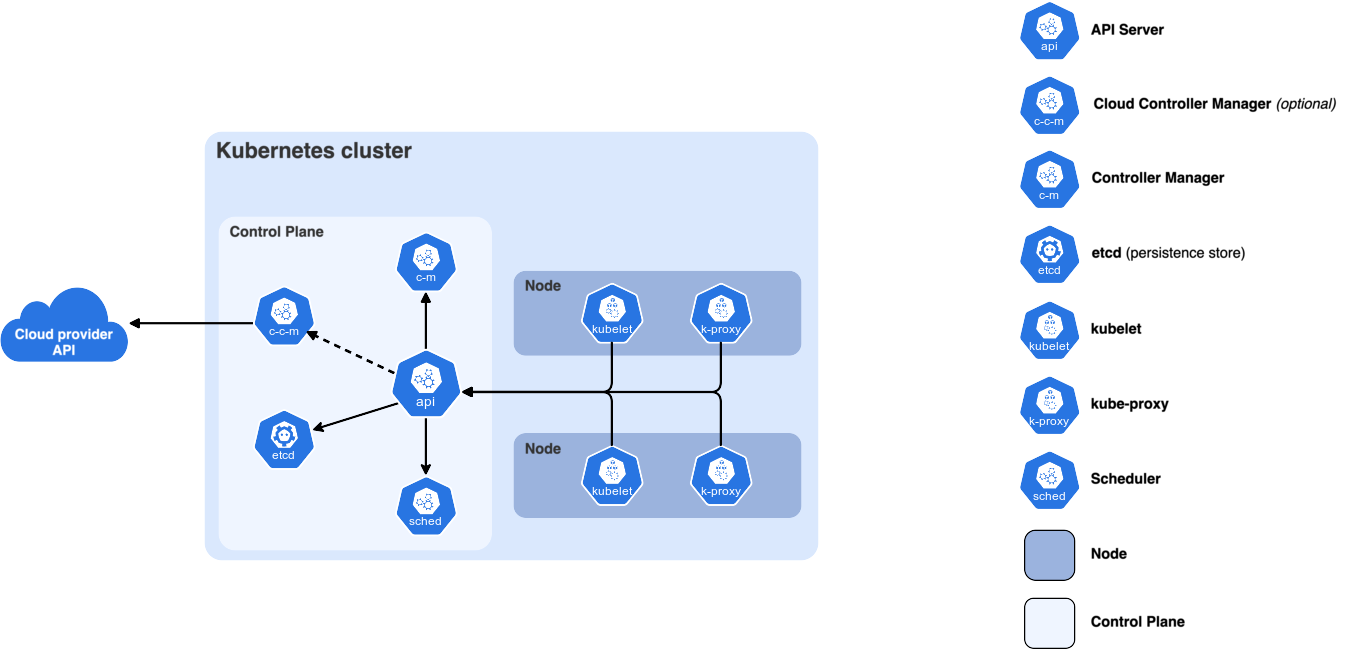
\includegraphics[width=\textwidth]{resources/k8s-architecture.png}
\caption{Arquitectura de Kubernetes}
\label{fig:k8s-architecture-svg}
\end{figure}

\begin{figure}[h]
\centering
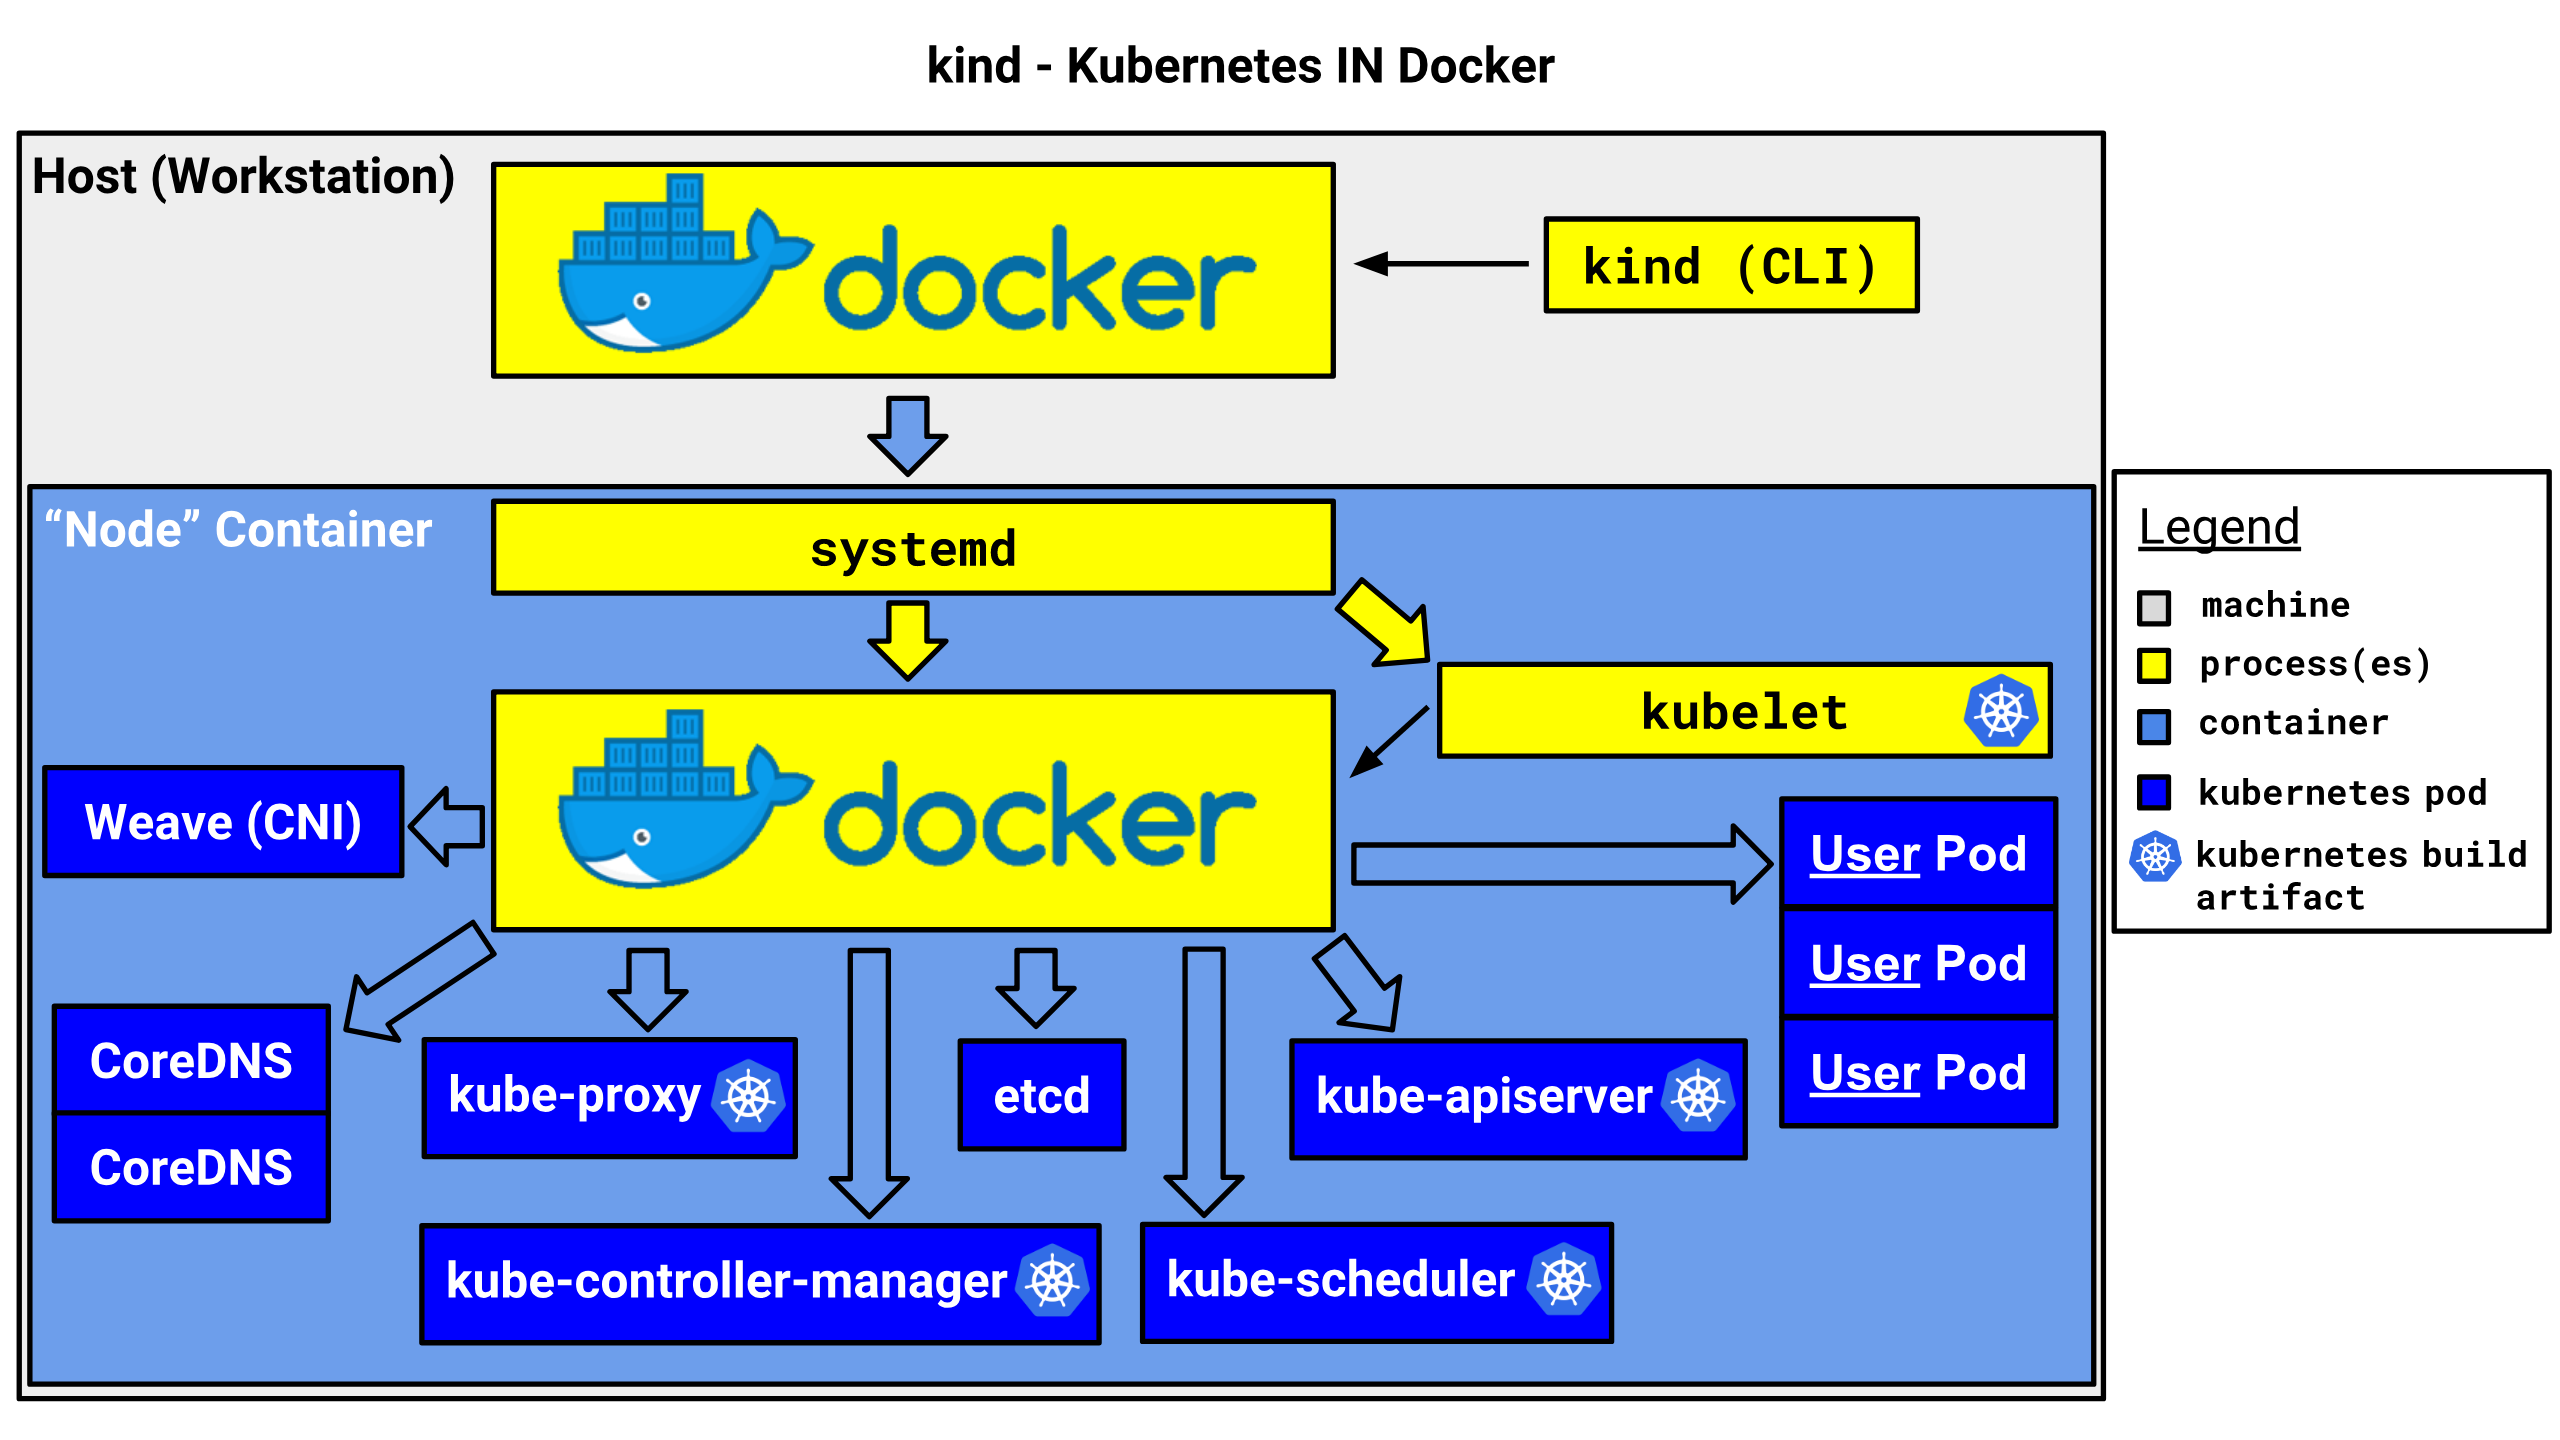
\includegraphics[width=\textwidth]{resources/kind-cluster-diagram.png}
\caption{Diagrama del clúster Kind}
\label{fig:kind-cluster-diagram}
\end{figure}

Esta configuración crea un cluster Kind con soporte para GPU mediante paso a través de dispositivos.

\subsection{Componentes}

\subsubsection{Nodos}

\begin{itemize}
    \item \textbf{Plano de Control}: 1 node ejecutando componentes de control de Kubernetes.
    \item \textbf{Trabajadores}: 4 nodes para cargas de trabajo de aplicaciones.
\end{itemize}

\subsubsection{Redes}

\begin{itemize}
    \item \textbf{CNI}: Kindnet (por defecto).
    \item \textbf{Puertos}: 12741-12761 expuestos en el plano de control para acceso externo.
    \item \textbf{Interna}: Red de pods 10.96.0.0/16.
\end{itemize}

\subsubsection{Acceso a GPU}

\begin{itemize}
    \item \textbf{Método}: Montajes de dispositivos + montajes de bibliotecas.
    \item \textbf{Dispositivos}: /dev/nvidia* (GPU, UVM, modeset, ctl).
    \item \textbf{Bibliotecas}: libnvidia-ml.so.1, libcuda.so.1.
    \item \textbf{Etiquetas}: nvidia.com/gpu.present=true en todos los nodos.
\end{itemize}

\subsubsection{Almacenamiento}

\begin{itemize}
    \item \textbf{CSI}: Clase de almacenamiento estándar (hostPath).
\end{itemize}

\subsection{Seguridad}

\begin{itemize}
    \item Acceso root en contenedores (por defecto en Kind).
    \item Acceso a dispositivos GPU mediante montajes.
    \item Sin modificaciones RBAC.
\end{itemize}

\subsection{Limitaciones}

\begin{itemize}
    \item Plano de control único para estabilidad.
    \item Programación de GPU mediante plugin de dispositivo (opcional).
    \item Sin volúmenes persistentes por defecto.
\end{itemize}

Con la arquitectura definida, el siguiente paso es la creación y configuración práctica del clúster Kind.

\newpage
\section{Creación y Configuración del Clúster}

\subsection{Creación del Clúster}

Utilice el archivo \texttt{config/kind-config.yaml}\footnote{En caso de no encontrar el archivo, puede crearlo usando el Anexo 6.} para crear el cluster:

\begin{lstlisting}
kind create cluster --config config/kind-config.yaml\footnote{En caso de no encontrar el archivo, puede crearlo usando el Anexo 6.}
\end{lstlisting}

\textbf{Qué crea:}
\begin{itemize}
    \item 1 nodo de plano de control.
    \item 4 nodos trabajadores.
    \item Puertos 12741-12761 expuestos en el plano de control.
    \item Dispositivos GPU montados en todos los nodos.
    \item Etiquetas de presencia de GPU.
\end{itemize}

\subsection{Eliminación del Clúster}

Si es necesario, elimine primero el cluster:

\begin{lstlisting}
kind delete cluster
\end{lstlisting}

\subsection{Verificación de Creación}

Verifique que el cluster se haya creado correctamente:

\begin{lstlisting}
kind get clusters
kubectl cluster-info
\end{lstlisting}

\subsection{Consideraciones Adicionales}

\begin{itemize}
    \item El clúster Kind es efímero por defecto; los datos se pierden al eliminar el clúster.
    \item Para persistencia, considere usar volúmenes hostPath o soluciones de almacenamiento externas.
    \item Monitoree el uso de recursos con herramientas como k9s o kubectl top.
    \item Para producción, evalúe clústeres reales en la nube o on-premises.
\end{itemize}

\newpage
\subsection{Configuracion de GPU}

\subsection{Montajes de Dispositivos}

\begin{figure}[h]
\centering
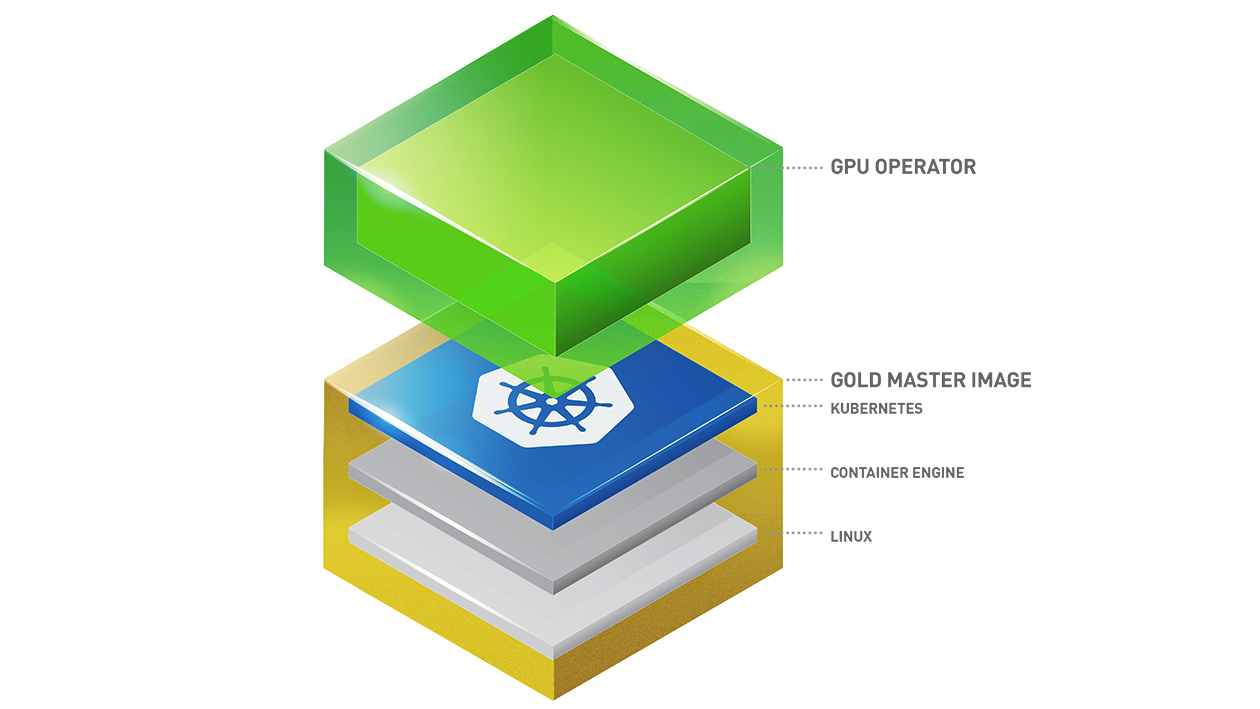
\includegraphics[width=\textwidth]{resources/gpu-operator-host_to_kubernetes.png}
\caption{Operador GPU: Host a Kubernetes}
\label{fig:gpu-operator}
\end{figure}

La configuracion monta:
\begin{itemize}
    \item Dispositivos \texttt{/dev/nvidia*}.
    \item Bibliotecas NVIDIA (\texttt{libnvidia-ml.so.1}, \texttt{libcuda.so.1}).
\end{itemize}

\subsection{Programación de GPU en Kubernetes}

Instale el plugin de dispositivo NVIDIA:

\begin{lstlisting}
kubectl apply -f https://raw.githubusercontent.com/NVIDIA/k8s-device-plugin/v0.17.0/deployments/static/nvidia-device-plugin.yml
\end{lstlisting}

Verifique recursos GPU:

\begin{lstlisting}
kubectl describe nodes | grep -A 5 nvidia.com/gpu
\end{lstlisting}

Una vez configurado el clúster y las GPUs, es crucial verificar que todo funcione correctamente antes de proceder al uso productivo.

\newpage
\section{Verificación y Pruebas}

Verifique el estado del cluster:

\begin{lstlisting}[caption={Verificación del estado del clúster}]
kubectl get nodes
kubectl get nodes --show-labels
kubectl cluster-info
\end{lstlisting}



Todos los nodos deben estar \texttt{Ready} con etiquetas de GPU.

\newpage
\section{Pruebas}

\subsection{Validacion de Acceso a GPU}

Ejecute comandos para probar el acceso a GPU:

\begin{lstlisting}[caption={Validación de acceso a GPU en nodos trabajadores}]
# Copiar nvidia-smi a trabajadores
docker cp /usr/bin/nvidia-smi kind-worker:/usr/bin/nvidia-smi
docker cp /usr/bin/nvidia-smi kind-worker2:/usr/bin/nvidia-smi
docker cp /usr/bin/nvidia-smi kind-worker3:/usr/bin/nvidia-smi
docker cp /usr/bin/nvidia-smi kind-worker4:/usr/bin/nvidia-smi

# Probar
docker exec kind-worker nvidia-smi
docker exec kind-worker2 nvidia-smi
docker exec kind-worker3 nvidia-smi
docker exec kind-worker4 nvidia-smi
\end{lstlisting}

Esperado: Información de GPU del host.

\begin{figure}[h]
\centering
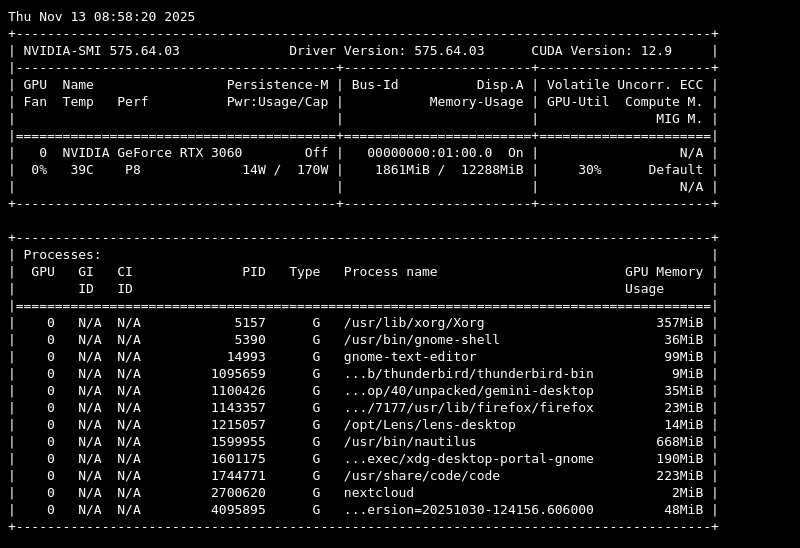
\includegraphics[width=\textwidth]{resources/results/nvidia_smi.png}
\caption{Salida de nvidia-smi en worker}
\end{figure}

\subsection{Prueba Automatizada}

Utilice \texttt{setup.sh}\footnote{En caso de no encontrar el script, puede crearlo usando el Anexo 1.} que incluye pruebas de GPU.

Si las pruebas pasan exitosamente, el clúster está listo para uso. En caso de problemas, consulte la siguiente sección de solución de problemas.

\newpage
\section{Solución de Problemas}

\subsection{Creación del Clúster Falla}

\begin{itemize}
    \item Asegúrese de que Docker esté ejecutándose: \texttt{sudo systemctl start docker}.
    \item Verifique información de Docker: \texttt{docker info}.
    \item Si hay tiempo de espera, simplifique la configuración (reduzca nodos).
\end{itemize}

\subsection{Nodos No Listos}

\begin{itemize}
    \item Espere 30-60 segundos después de la creación.
    \item Verifique CNI: \texttt{kubectl get pods -n kube-system}.
\end{itemize}

\subsection{GPU No Detectada}

\begin{itemize}
    \item Verifique que el host tenga drivers NVIDIA: \texttt{nvidia-smi}.
    \item Verifique montajes en la configuración.
    \item Para programar GPU en Kubernetes, el plugin de dispositivo debe ejecutarse.
\end{itemize}

\subsection{Problemas de Exposición de Puertos}

\begin{itemize}
    \item Los puertos 12741-12761 están expuestos en el plano de control.
    \item Use \texttt{docker ps} para verificar mapeos.
\end{itemize}

\subsection{Errores del Plugin de Dispositivo}

\begin{itemize}
    \item "demasiados archivos abiertos": Aumente ulimits o omita el plugin.
    \item Use montajes directos para acceso a GPU.
\end{itemize}

\subsection{Recrear Clúster}

\begin{lstlisting}
kind delete cluster
kind create cluster --config kind-config.yaml\footnote{En caso de no encontrar el archivo, puede crearlo usando el Anexo 6.}
\end{lstlisting}

\newpage
\section{Limpieza y Mantenimiento}

\begin{lstlisting}
./scripts/cleanup.sh
# Or manually:
kind delete cluster
\end{lstlisting}\footnote{En caso de no encontrar el script, puede crearlo usando el Anexo 3.}

Para consultas comunes y consejos adicionales, consulte las preguntas frecuentes a continuación.

\newpage
\section{Preguntas Frecuentes}

\subsection{General}

\textbf{¿Por qué Kind?} \\
Kind proporciona clusteres ligeros de Kubernetes para desarrollo/pruebas con soporte para GPU.

\textbf{¿Por qué no minikube?} \\
Kind soporta mejor clusteres multi-nodo y paso a través de GPU.

\subsection{Configuracion}

\textbf{¿La creación del cluster se agota?} \\
Reduzca nodos en la configuración o aumente el tiempo de espera. Use 1 plano de control + menos trabajadores.

\textbf{¿Docker no encontrado?} \\
Asegúrese de que el daemon Docker esté ejecutándose: \texttt{sudo systemctl start docker}.

\textbf{¿GPU no detectada?} \\
Verifique drivers del host con \texttt{nvidia-smi}. Asegúrese de que los montajes en la configuración coincidan con las rutas del host.

\subsection{GPU}

\textbf{¿El plugin de dispositivo falla?} \\
Use montajes directos para acceso. El plugin requiere drivers NVIDIA en los nodos (no presentes).

\textbf{¿Cómo programar pods GPU?} \\
Use nodeSelector: \texttt{nvidia.com/gpu.present: "true"}.

\textbf{¿Múltiples GPUs?} \\
La configuración monta /dev/nvidia0; ajuste para más GPUs.

\subsection{Uso}

\textbf{¿Cómo acceder a servicios?} \\
Use puertos expuestos 12741-12761 en localhost.

\textbf{¿Almacenamiento persistente?} \\
Use volúmenes hostPath o agregue drivers CSI.

\textbf{¿Agregar más nodos?} \\
No soportado; recree el cluster con nueva configuración.

\subsection{Solucion de Problemas}

\textbf{¿Nodos no Ready?} \\
Espere 1-2 minutos. Verifique pods CNI: \texttt{kubectl get pods -n kube-system}.

\textbf{¿kubectl conexión rechazada?} \\
Ejecute \texttt{kind export kubeconfig} o verifique estado del cluster con \texttt{kind get clusters}.

Para ilustrar el uso práctico del clúster, a continuación se presentan ejemplos detallados de despliegues y operaciones comunes.

\newpage
\section{Ejemplos de Uso}

\subsection{Ejecutar Pod GPU}

\begin{figure}[h]
\centering
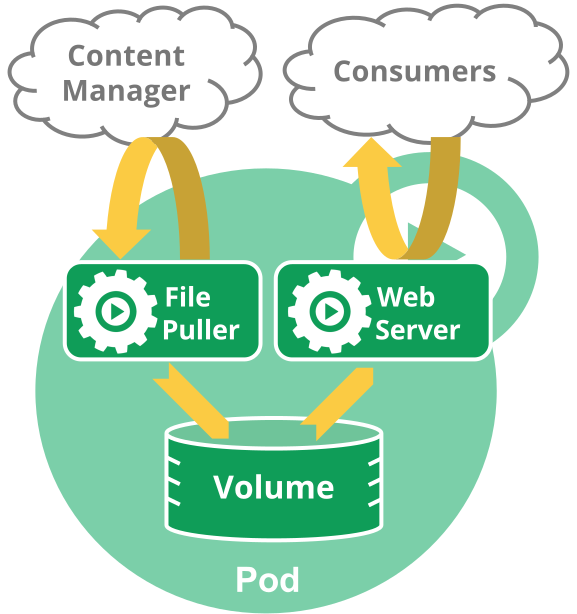
\includegraphics[width=\textwidth]{resources/pod-overview.png}
\caption{Diagrama de un Pod en Kubernetes}
\label{fig:pod-diagram}
\end{figure}

\begin{lstlisting}
kubectl apply -f examples/gpu-pod-example.yaml
kubectl logs gpu-pod
\end{lstlisting}

El archivo YAML del ejemplo:

\begin{lstlisting}
apiVersion: v1
kind: Pod
metadata:
  name: gpu-pod
spec:
  nodeSelector:
    nvidia.com/gpu.present: "true"
  containers:
  - name: gpu-container
    image: nvidia/cuda:12.2.0-base-ubuntu22.04
    command: ["nvidia-smi"]
    resources:
      limits:
        nvidia.com/gpu: 1  # Solicitar 1 GPU (si el plugin funciona)
  restartPolicy: Never
\end{lstlisting}

\subsection{Ejemplo de Despliegue de una Aplicación Simple}

Este ejemplo demuestra cómo desplegar una aplicación web simple en el clúster Kind. Sirve para verificar que el clúster está funcionando correctamente y para practicar comandos básicos de Kubernetes.

\begin{lstlisting}
kubectl create deployment hello-world --image=gcr.io/google-samples/hello-app:1.0
kubectl expose deployment hello-world --type=LoadBalancer --port=8080
kubectl get services
\end{lstlisting}

\subsection{Ejemplo de Uso de GPU para Computación Científica}

Este ejemplo muestra cómo ejecutar un contenedor que utiliza CUDA para cálculos científicos. Sirve para validar el soporte de GPU en el clúster y demostrar el uso de recursos GPU en aplicaciones de alto rendimiento.

\begin{lstlisting}
apiVersion: v1
kind: Pod
metadata:
  name: cuda-vector-add
spec:
  nodeSelector:
    nvidia.com/gpu.present: "true"
  containers:
  - name: cuda-vector-add
    image: nvcr.io/nvidia/k8s/cuda-sample:vectoradd-cuda10.2
    resources:
      limits:
        nvidia.com/gpu: 1
  restartPolicy: Never
\end{lstlisting}

\subsection{Ejemplo de Escalado de Pods}

Este ejemplo ilustra cómo escalar una aplicación para manejar más carga. Sirve para aprender sobre la escalabilidad horizontal en Kubernetes y cómo ajustar recursos dinámicamente.

\begin{lstlisting}
kubectl scale deployment hello-world --replicas=3
kubectl get pods
\end{lstlisting}

\subsection{Ejemplo de Monitoreo con k9s}

Este ejemplo explica cómo usar k9s para monitorear el estado del clúster en tiempo real. Sirve para facilitar la observación y debugging de aplicaciones en Kubernetes sin comandos complejos.

\begin{lstlisting}
k9s
# Dentro de k9s: presiona 'p' para ver pods, 'd' para deployments
\end{lstlisting}

\subsection{Ejemplo de Despliegue con ArgoCD}

Este ejemplo muestra cómo desplegar una aplicación usando GitOps con ArgoCD. Sirve para automatizar despliegues continuos y mantener la sincronización entre código y clúster.

\begin{lstlisting}
kubectl apply -f argocd-app.yaml
\end{lstlisting}

Donde \texttt{argocd-app.yaml} contiene:

\begin{lstlisting}
apiVersion: argoproj.io/v1alpha1
kind: Application
metadata:
  name: my-app
  namespace: argocd
spec:
  project: default
  source:
    repoURL: https://github.com/my-org/my-app
    targetRevision: HEAD
    path: .
  destination:
    server: https://kubernetes.default.svc
    namespace: default
\end{lstlisting}

\subsection{Ejemplo de Configuración de Recursos GPU Avanzada}

Este ejemplo demuestra cómo configurar límites y solicitudes de GPU para múltiples contenedores. Sirve para optimizar el uso de recursos GPU en aplicaciones complejas con múltiples componentes.

\begin{lstlisting}
apiVersion: v1
kind: Pod
metadata:
  name: multi-gpu-pod
spec:
  nodeSelector:
    nvidia.com/gpu.present: "true"
  containers:
  - name: gpu-container-1
    image: nvidia/cuda:12.2.0-base-ubuntu22.04
    resources:
      limits:
        nvidia.com/gpu: 1
      requests:
        nvidia.com/gpu: 1
  - name: gpu-container-2
    image: nvidia/cuda:12.2.0-base-ubuntu22.04
    resources:
      limits:
        nvidia.com/gpu: 1
      requests:
        nvidia.com/gpu: 1
  restartPolicy: Never
\end{lstlisting}

\subsection{Ejemplo de Debugging de Pods con GPU}

Este ejemplo muestra comandos para diagnosticar problemas en pods que usan GPU. Sirve para solucionar issues comunes como fallos de asignación de GPU o errores de contenedores.

\begin{lstlisting}
kubectl describe pod gpu-pod
kubectl logs gpu-pod
kubectl exec -it gpu-pod -- nvidia-smi
\end{lstlisting}

\subsection{Ejemplo de Backup y Restauración de Configuración}

Este ejemplo ilustra cómo hacer backup de la configuración del clúster. Sirve para preservar configuraciones importantes y facilitar la recuperación en caso de fallos.

\begin{lstlisting}
kubectl get all --all-namespaces -o yaml > cluster-backup.yaml
# Para restaurar: kubectl apply -f cluster-backup.yaml
\end{lstlisting}

Además de los ejemplos básicos, el proyecto incluye herramientas adicionales para mejorar la experiencia de gestión del clúster.

\newpage
\section{Herramientas Adicionales}

\subsubsection{Instalacion de ArgoCD}

\begin{figure}[h]
\begin{center}

\includegraphics[width=0.3\textwidth]{resources/argocd-logo-converted.png}
\caption{Logo de ArgoCD}
\label{fig:argocd-logo}
\end{center}
\end{figure}

ArgoCD es una herramienta GitOps para Kubernetes.

\begin{figure}[h]
\centering
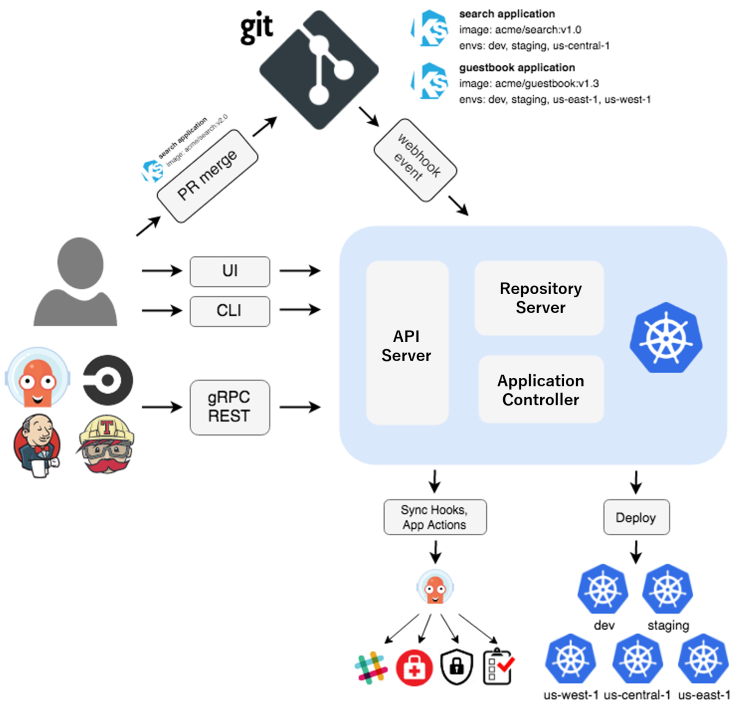
\includegraphics[width=\textwidth]{resources/argocd-architecture.png}
\caption{Arquitectura de ArgoCD}
\label{fig:argocd-architecture}
\end{figure}

\begin{lstlisting}[caption={Instalación de ArgoCD en el clúster}]
kubectl create namespace argocd
kubectl apply -n argocd -f https://raw.githubusercontent.com/argoproj/argo-cd/stable/manifests/install.yaml
\end{lstlisting}

Espere a que los pods estén listos:

\begin{lstlisting}[caption={Verificación de pods de ArgoCD}]
kubectl get pods -n argocd
\end{lstlisting}

Acceda a ArgoCD:

\begin{lstlisting}[caption={Acceso a la interfaz web de ArgoCD}]
kubectl port-forward svc/argocd-server -n argocd 8080:443
\end{lstlisting}

Abra https://localhost:8080

\begin{figure}[h]
\centering
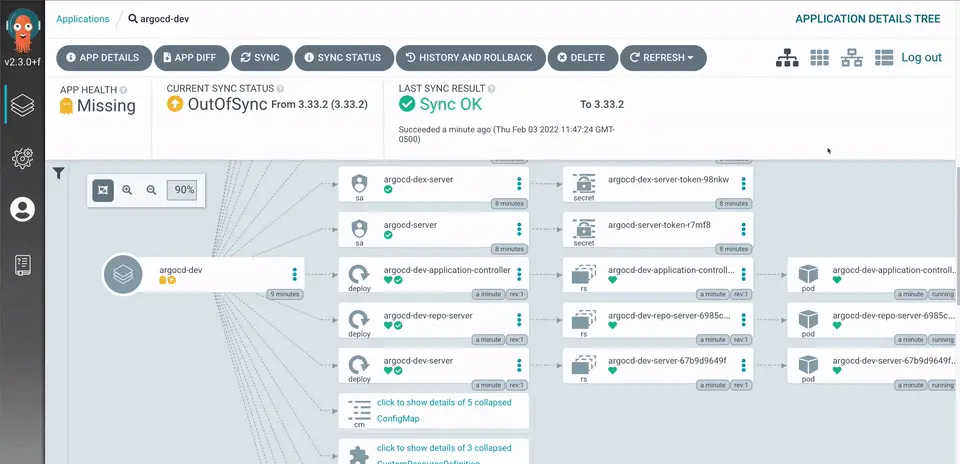
\includegraphics[width=\textwidth]{resources/argocd-ui.png}
\caption{Interfaz de usuario de ArgoCD}
\label{fig:argocd-ui}
\end{figure}

Credenciales:
\begin{itemize}
    \item Usuario: admin
    \item Contraseña: \texttt{kubectl -n argocd get secret argocd-initial-admin-secret -o jsonpath="{.data.password}" | base64 -d}
\end{itemize}

\subsubsection{Instalacion de k9s}

\begin{figure}[h]
\begin{center}
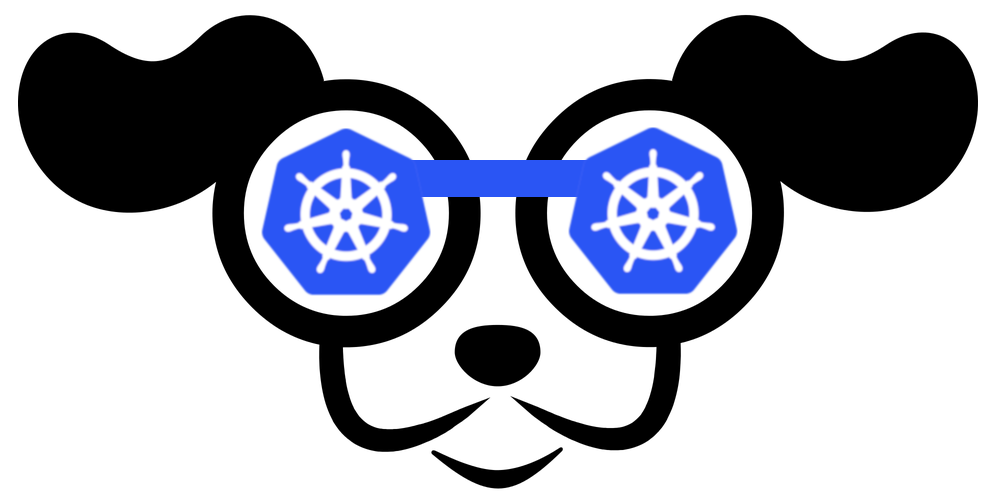
\includegraphics[width=0.3\textwidth]{resources/k9s-logo.png}
\caption{Logo de k9s}
\label{fig:k9s-logo}
\end{center}
\end{figure}

k9s es una interfaz de usuario basada en terminal para gestionar clústeres de Kubernetes de manera eficiente. Proporciona una experiencia interactiva para navegar por recursos, logs, pods y más, sin necesidad de comandos complejos de kubectl.

\begin{figure}[h]
\centering
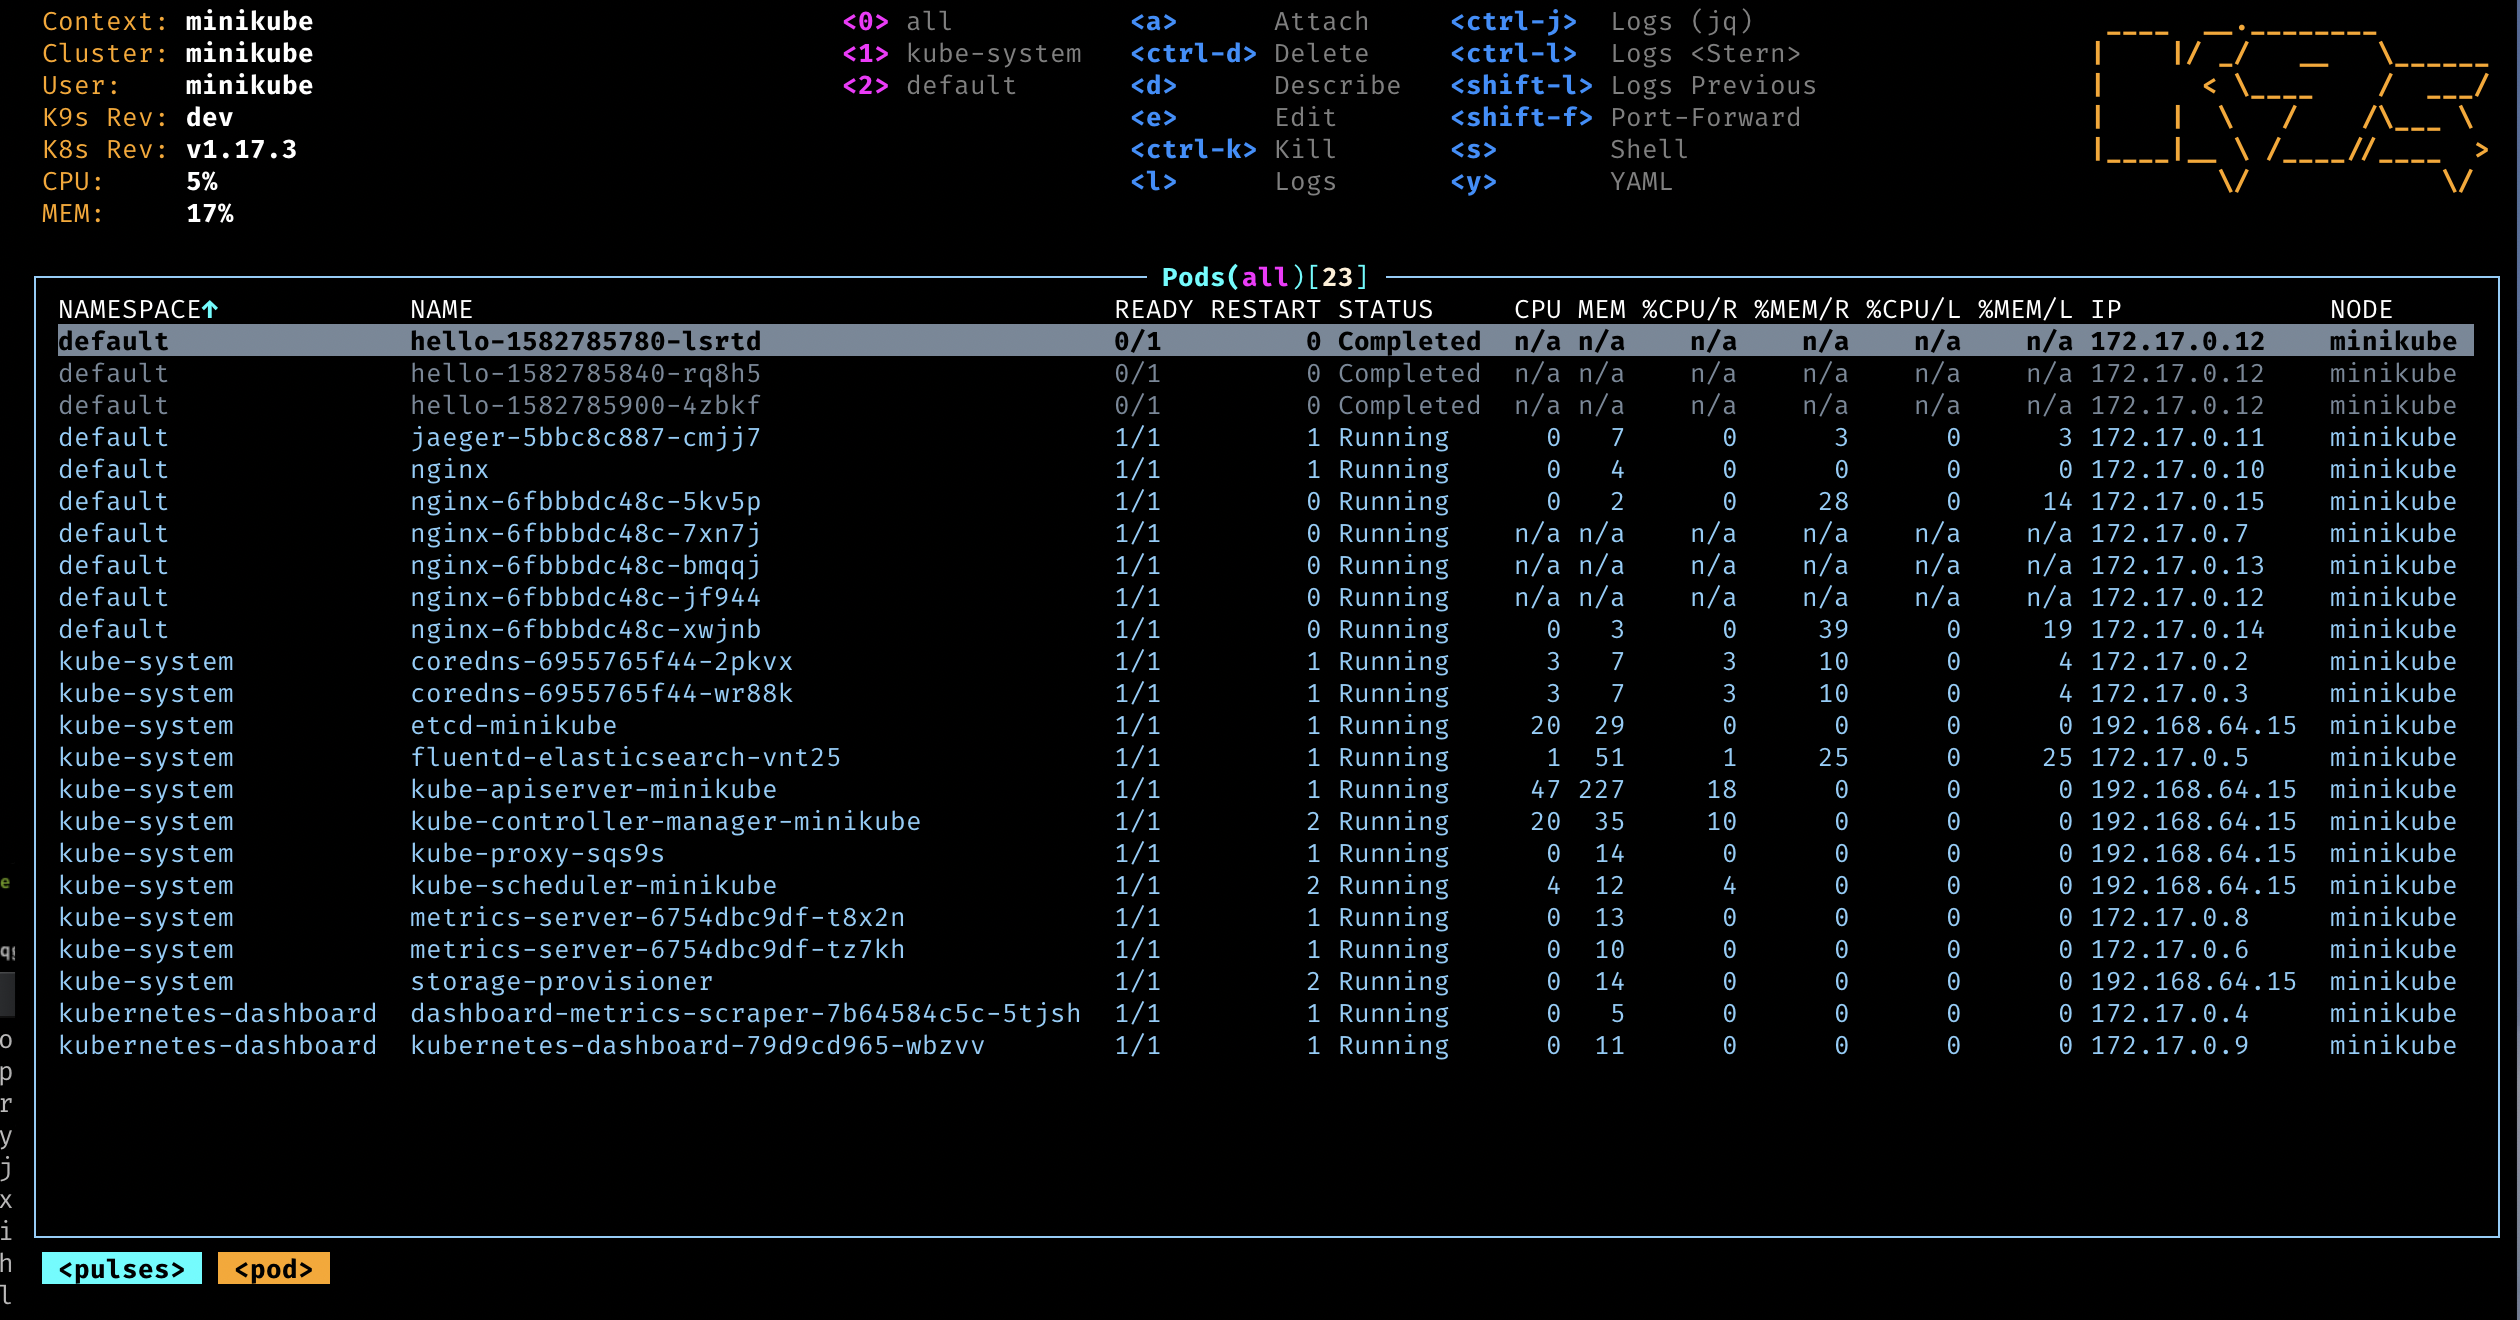
\includegraphics[width=\textwidth]{resources/k9s-screenshot.png}
\caption{Captura de pantalla de k9s}
\label{fig:k9s-screenshot}
\end{figure}

\begin{itemize}
    \item \textbf{Ventajas:} Navegación rápida con atajos de teclado, vistas en tiempo real, y comandos integrados para operaciones comunes.
    \item \textbf{Uso:} Ideal para monitoreo y debugging en entornos de desarrollo.
\end{itemize}

Instalación:

\begin{lstlisting}[caption={Descarga e instalación de k9s}]
# Descargar la última versión
curl -Lo ./k9s.tar.gz https://github.com/derailed/k9s/releases/latest/download/k9s_Linux_amd64.tar.gz

# Extraer
tar -xzf k9s.tar.gz

# Hacer ejecutable
chmod +x k9s

# Mover a directorio en PATH
mkdir -p ~/bin
mv k9s ~/bin/
\end{lstlisting}

Agregar a PATH (temporalmente):

\begin{lstlisting}[caption={Configuración temporal de PATH para k9s}]
source scripts/set_path.sh
\end{lstlisting}

O permanentemente:

\begin{lstlisting}[caption={Configuración permanente de PATH para k9s}]
echo 'export PATH="$PATH:$HOME/bin"' >> ~/.bashrc
source ~/.bashrc
\end{lstlisting}\footnote{En caso de no encontrar el script, puede crearlo usando el Anexo 5.}

Ejecutar k9s:

\begin{lstlisting}[caption={Ejecución de k9s}]
k9s
\end{lstlisting}

k9s detecta automáticamente el contexto kubeconfig actual y se conecta al clúster. Use las teclas de navegación para explorar recursos como pods, servicios y deployments. Presione \texttt{?} para ver la ayuda integrada.

\subsubsection{Integración con Lens}



Lens es una interfaz gráfica (GUI) para gestionar clústeres de Kubernetes, proporcionando una experiencia visual intuitiva similar a un IDE. Permite visualizar recursos, editar YAML, ver logs en tiempo real y gestionar aplicaciones sin necesidad de línea de comandos.

\begin{figure}[h]
\centering
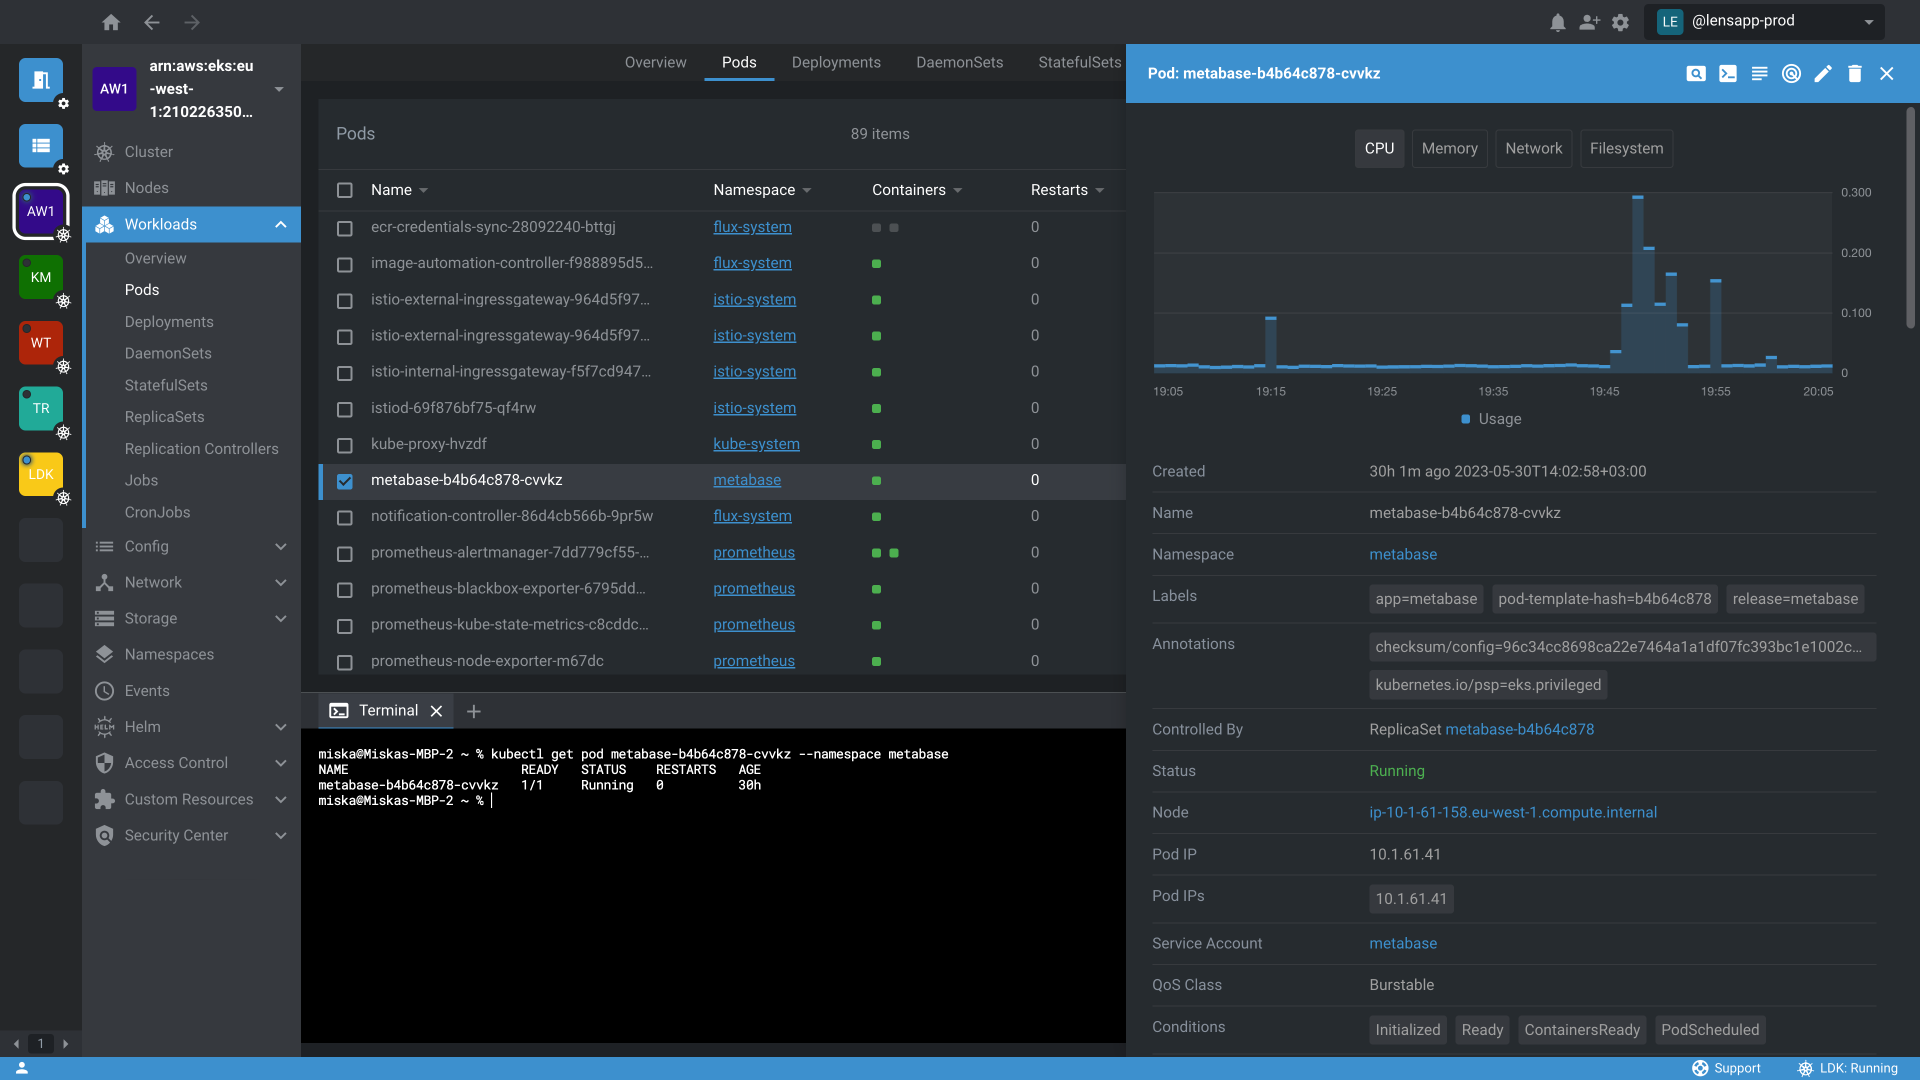
\includegraphics[width=\textwidth]{resources/lens-screenshot.png}
\caption{Captura de pantalla de Lens}
\label{fig:lens-screenshot}
\end{figure}

\begin{itemize}
    \item \textbf{Ventajas:} Interfaz amigable para principiantes, integración con Helm, y soporte para múltiples clústeres.
    \item \textbf{Uso:} Perfecto para usuarios que prefieren una interfaz gráfica sobre la terminal.
\end{itemize}

Instalación de Lens:

Basado en: \url{https://docs.k8slens.dev/getting-started/install-lens/}

\begin{lstlisting}
# Descargar el paquete .deb (para Ubuntu/Debian)
curl -LO https://api.k8slens.dev/binaries/Lens-2023.12.121249-latest.amd64.deb

# Instalar
sudo dpkg -i Lens-2023.12.121249-latest.amd64.deb

# Resolver dependencias si es necesario
sudo apt install -f
\end{lstlisting}

Alternativamente, descargar desde el sitio web oficial y seguir las instrucciones para Linux.

Configuración con el clúster Kind:

Primero, obtener el archivo de configuración del clúster:

\begin{lstlisting}
kind get kubeconfig > config/kubeconfig.yaml
\end{lstlisting}

En Lens:

\begin{enumerate}
    \item Abra Lens.
    \item Haga clic en "Add Cluster" o "Import Cluster".
    \item Seleccione "From kubeconfig" y elija \texttt{config/kubeconfig.yaml}.
    \item El clúster aparecerá en la lista; selecciónelo para conectarse.
\end{enumerate}

Una vez conectado, puede explorar nodos, pods, servicios y más a través de la interfaz gráfica. Lens también permite instalar extensiones y gestionar Helm charts.

\newpage
\section{Registro de Cambios}

Todas las modificaciones notables a este proyecto se documentarán en este archivo.

El formato se basa en \href{https://keepachangelog.com/en/1.0.0/}{Keep a Changelog}, y este proyecto adhiere a \href{https://semver.org/spec/v2.0.0.html}{Versionado Semántico}.

\subsection{[1.1.0] - 2025-11-13}

\subsubsection{Agregado}
\begin{tabularx}{\textwidth}{l X}
Agregado & Mega setup script (mega\_setup.sh) para configuración automatizada completa. \\
\end{tabularx}

\subsubsection{Características}
\begin{itemize}
    \item Validación de acceso GPU en todos los trabajadores.
    \item Documentación profesional.
    \item Scripts de limpieza.
\end{itemize}

\subsection{[1.0.0] - 2025-11-12}

\subsubsection{Agregado}
\begin{tabularx}{\textwidth}{l X}
Agregado & Configuración inicial para clúster Kind con soporte GPU. \\
 & Scripts automatizados para instalación y pruebas. \\
 & Configuración para 1 plano de control + 4 trabajadores. \\
 & Exposición de puertos (12741-12761). \\
 & Montaje de dispositivos GPU y etiquetado. \\
 & Guias de validación y solucion de problemas. \\
 & Makefile para automatizacion. \\
 & Ejemplo de pod GPU en YAML. \\
\end{tabularx}

\subsubsection{Características}
\begin{itemize}
    \item Validacion de acceso GPU en todos los trabajadores.
    \item Documentacion profesional.
    \item Scripts de limpieza.
\end{itemize}

\newpage
\section{Licencia}

Este proyecto está licenciado bajo la Licencia MIT - consulte el archivo LICENSE para detalles.

\begin{verbatim}
MIT License

Copyright (c) 2025 Kind GPU Setup

Permission is hereby granted, free of charge, to any person obtaining a copy
of this software and associated documentation files (the "Software"), to deal
in the Software without restriction, including without limitation the rights
to use, copy, modify, merge, publish, distribute, sublicense, and/or sell
copies of the Software, and to permit persons to whom the Software is
furnished to do so, subject to the following conditions:

The above copyright notice and this permission notice shall be included in all
copies or substantial portions of the Software.

THE SOFTWARE IS PROVIDED "AS IS", WITHOUT WARRANTY OF ANY KIND, EXPRESS OR
IMPLIED, INCLUDING BUT NOT LIMITED TO THE WARRANTIES OF MERCHANTABILITY,
FITNESS FOR A PARTICULAR PURPOSE AND NONINFRINGEMENT. IN NO EVENT SHALL THE
AUTHORS OR COPYRIGHT HOLDERS BE LIABLE FOR ANY CLAIM, DAMAGES OR OTHER
LIABILITY, WHETHER IN AN ACTION OF CONTRACT, TORT OR OTHERWISE, ARISING FROM,
OUT OF OR IN CONNECTION WITH THE SOFTWARE OR THE USE OR OTHER DEALINGS IN THE
SOFTWARE.
\end{verbatim}

\newpage
\section{Apéndices}

\subsection{Versión de Componentes}

\begin{tabularx}{\textwidth}{l l X}
Componente & Versión & Descripción \\
Kind & v0.30.0 & Herramienta para ejecutar clusters Kubernetes locales usando contenedores Docker. \\
Kubernetes & v1.34.0 (kindest/node) & Plataforma de orquestación de contenedores utilizada en el cluster. \\
Driver NVIDIA & 575.64.03 & Controlador para GPUs NVIDIA, necesario para el acceso a hardware GPU. \\
CUDA & 12.9 & Plataforma de computación paralela y modelo de programación de NVIDIA. \\
Plugin de Dispositivo NVIDIA & v0.17.0 & Plugin de Kubernetes para gestionar recursos GPU en pods. \\
\end{tabularx}

\subsection{Estructura del Proyecto}

\begin{lstlisting}[caption={Estructura del proyecto}]
kind_use/
- argocd-app.yaml          # Configuracion de aplicacion ArgoCD
- config/
  - kind-config.yaml      # Configuracion del cluster
  - kubeconfig.yaml       # Kubeconfig para herramientas externas
- docs/
  - documentation.tex     # Documentacion en LaTeX
  - documentation.pdf     # Documentacion compilada
  - README.md             # Esta guia
  - architecture.md       # Arquitectura del sistema
  - requirements.md       # Prerrequisitos
  - FAQ.md                # Preguntas frecuentes
  - troubleshooting.md    # Guia de solucion de problemas
  - CHANGELOG.md          # Historial de cambios
  - *.txt                 # Archivos de referencia de comandos
  - resources/            # Recursos (imagenes, resultados)
- examples/
  - gpu-pod-example.yaml  # Ejemplo de pod GPU
- scripts/
  - setup.sh              # Configuracion automatizada basica
  - cleanup.sh            # Script de limpieza
  - validate.sh           # Verificacion de prerrequisitos
  - monitoring.sh         # Monitoreo del cluster
  - set_path.sh           # Configuracion de PATH
  - mega_setup.sh         # Configuracion automatizada completa
  - cluster_manager.py    # Gestor de cluster en Python
  - gpu_monitor.py        # Monitor de recursos GPU
- .gitignore                # Reglas de ignorar Git
- LICENSE                   # Licencia MIT
- Makefile                  # Objetivos de automatizacion
- versions.txt              # Informacion de versiones
\end{lstlisting}

\section{Anexos}

Este apartado contiene los scripts y archivos de configuración utilizados en la documentación. Cada anexo incluye el contenido completo del archivo correspondiente, con explicaciones de su propósito y uso.

\subsection{16.1: Script setup.sh}

Este script automatiza la instalación y configuración de Docker, NVIDIA Container Toolkit, kubectl, containerd, etcd, kubelet y Kind, facilitando la preparación del entorno para el cluster Kubernetes local.

\begin{lstlisting}[language=bash]
#!/bin/bash

# Setup script for Kind cluster with GPU

echo "Installing Kind..."
curl -Lo ./kind https://kind.sigs.k8s.io/dl/v0.30.0/kind-linux-amd64
chmod +x ./kind
sudo mv ./kind /usr/local/bin/kind

echo "Creating cluster..."
kind create cluster --config kind-config.yaml\footnote{En caso de no encontrar el archivo, puede crearlo usando el Anexo 6.}

echo "Verifying cluster..."
kubectl get nodes

echo "Setting up GPU labels..."
kubectl label node kind-control-plane nvidia.com/gpu.present=true
kubectl label node kind-worker kind-worker2 kind-worker3 kind-worker4 nvidia.com/gpu.present=true

echo "Installing NVIDIA device plugin..."
kubectl apply -f https://raw.githubusercontent.com/NVIDIA/k8s-device-plugin/v0.17.0/deployments/static/nvidia-device-plugin.yml

echo "Testing GPU on workers..."
docker cp /usr/bin/nvidia-smi kind-worker:/usr/bin/nvidia-smi
docker cp /usr/bin/nvidia-smi kind-worker2:/usr/bin/nvidia-smi
docker cp /usr/bin/nvidia-smi kind-worker3:/usr/bin/nvidia-smi
docker cp /usr/bin/nvidia-smi kind-worker4:/usr/bin/nvidia-smi

docker exec kind-worker nvidia-smi
docker exec kind-worker2 nvidia-smi
docker exec kind-worker3 nvidia-smi
docker exec kind-worker4 nvidia-smi

echo "Setup complete!"
\end{lstlisting}

Este script verifica que todos los prerrequisitos del sistema estén cumplidos antes de proceder con la creación del cluster, incluyendo la presencia de herramientas instaladas y configuraciones correctas.

\subsection{16.2: Script validate.sh}

\begin{lstlisting}[language=bash]
#!/bin/bash

# Validation script for prerequisites

echo "Validating prerequisites..."

# Check Docker
if ! docker info > /dev/null 2>&1; then
    echo "ERROR: Docker not running or not installed"
    exit 1
fi
echo "OK: Docker OK"

# Check NVIDIA
if ! nvidia-smi > /dev/null 2>&1; then
    echo "ERROR: NVIDIA GPU/drivers not available"
    exit 1
fi
echo "OK: NVIDIA GPU OK"

# Check sudo
if ! sudo -n true 2>/dev/null; then
    echo "WARNING: Sudo may require password"
fi

# Check if Kind exists
if command -v kind > /dev/null 2>&1; then
    echo "OK: Kind installed: $(kind --version)"
else
    echo "WARNING: Kind not installed, run install_kind.txt"
fi

# Check kubectl
if command -v kubectl > /dev/null 2>&1; then
    echo "OK: kubectl installed"
else
    echo "WARNING: kubectl not installed"
fi

echo "Validation complete!"
\end{lstlisting}

\subsection{16.3: Script cleanup.sh}

\begin{lstlisting}[language=bash]
#!/bin/bash

# Cleanup script

echo "Deleting cluster..."
kind delete cluster

echo "Removing Kind binary..."
sudo rm /usr/local/bin/kind

echo "Cleanup complete!"
\end{lstlisting}

\subsection{16.4: Script monitoring.sh}

\begin{lstlisting}[language=bash]
#!/bin/bash

# Monitoring script for cluster status

echo "=== Cluster Status ==="
kubectl get nodes -o wide

echo -e "\n=== Pod Status ==="
kubectl get pods -A --no-headers | wc -l
kubectl get pods -A | grep -v Running

echo -e "\n=== GPU Resources ==="
kubectl describe nodes | grep -A 5 "nvidia.com/gpu"

echo -e "\n=== Exposed Ports ==="
docker ps | grep kind-control-plane | grep -o "127[0-9]*->"

echo -e "\n=== Disk Usage ==="
df -h | grep -E "(docker|overlay)"

echo -e "\n=== Disk Usage ==="
df -h | grep -E "(docker|overlay)"

echo "Monitoring complete."
\end{lstlisting}

\subsection{16.5: Script set\_path.sh}

\begin{lstlisting}[language=bash]
#!/bin/bash

# Script to add ~/bin to PATH

export PATH="$PATH:$HOME/bin"
echo "Added ~/bin to PATH. Run 'source set_path.sh' or add to ~/.bashrc"
\end{lstlisting}

\newpage
\subsection{16.6: Archivo kind-config.yaml}

\begin{lstlisting}
kind: Cluster
apiVersion: kind.x-k8s.io/v1alpha4
nodes:
- role: control-plane
  extraPortMappings:
  - containerPort: 80
    hostPort: 12741
    listenAddress: "127.0.0.1"
  - containerPort: 81
    hostPort: 12742
    listenAddress: "127.0.0.1"
  - containerPort: 82
    hostPort: 12743
    listenAddress: "127.0.0.1"
  - containerPort: 83
    hostPort: 12744
    listenAddress: "127.0.0.1"
  - containerPort: 84
    hostPort: 12745
    listenAddress: "127.0.0.1"
  - containerPort: 85
    hostPort: 12746
    listenAddress: "127.0.0.1"
  - containerPort: 86
    hostPort: 12747
    listenAddress: "127.0.0.1"
  - containerPort: 87
    hostPort: 12748
    listenAddress: "127.0.0.1"
  - containerPort: 88
    hostPort: 12749
    listenAddress: "127.0.0.1"
  - containerPort: 89
    hostPort: 12750
    listenAddress: "127.0.0.1"
  - containerPort: 90
    hostPort: 12751
    listenAddress: "127.0.0.1"
  - containerPort: 91
    hostPort: 12752
    listenAddress: "127.0.0.1"
  - containerPort: 92
    hostPort: 12753
    listenAddress: "127.0.0.1"
  - containerPort: 93
    hostPort: 12754
    listenAddress: "127.0.0.1"
  - containerPort: 94
    hostPort: 12755
    listenAddress: "127.0.0.1"
  - containerPort: 95
    hostPort: 12756
    listenAddress: "127.0.0.1"
  - containerPort: 96
    hostPort: 12757
    listenAddress: "127.0.0.1"
  - containerPort: 97
    hostPort: 12758
    listenAddress: "127.0.0.1"
  - containerPort: 98
    hostPort: 12759
    listenAddress: "127.0.0.1"
  - containerPort: 99
    hostPort: 12760
    listenAddress: "127.0.0.1"
  - containerPort: 100
    hostPort: 12761
    listenAddress: "127.0.0.1"
  extraMounts:
  - hostPath: /dev/nvidia0
    containerPath: /dev/nvidia0
  - hostPath: /dev/nvidiactl
    containerPath: /dev/nvidiactl
  - hostPath: /dev/nvidiamodeset
    containerPath: /dev/nvidiamodeset
  - hostPath: /dev/nvidia-uvm
    containerPath: /dev/nvidia-uvm
  - hostPath: /dev/nvidia-uvm-tools
    containerPath: /dev/nvidia-uvm-tools
  - hostPath: /usr/lib/x86_64-linux-gnu/libnvidia-ml.so.1
    containerPath: /usr/lib/x86_64-linux-gnu/libnvidia-ml.so.1
  - hostPath: /usr/lib/x86_64-linux-gnu/libcuda.so.1
    containerPath: /usr/lib/x86_64-linux-gnu/libcuda.so.1
  kubeadmConfigPatches:
  - |
    kind: InitConfiguration
    nodeRegistration:
      kubeletExtraArgs:
        node-labels: "nvidia.com/gpu.present=true"
- role: worker
  extraMounts:
  - hostPath: /dev/nvidia0
    containerPath: /dev/nvidia0
  - hostPath: /dev/nvidiactl
    containerPath: /dev/nvidiactl
  - hostPath: /dev/nvidiamodeset
    containerPath: /dev/nvidiamodeset
  - hostPath: /dev/nvidia-uvm
    containerPath: /dev/nvidia-uvm
  - hostPath: /dev/nvidia-uvm-tools
    containerPath: /dev/nvidia-uvm-tools
  - hostPath: /usr/lib/x86_64-linux-gnu/libnvidia-ml.so.1
    containerPath: /usr/lib/x86_64-linux-gnu/libnvidia-ml.so.1
  - hostPath: /usr/lib/x86_64-linux-gnu/libcuda.so.1
    containerPath: /usr/lib/x86_64-linux-gnu/libcuda.so.1
- role: worker
  extraMounts:
  - hostPath: /dev/nvidia0
    containerPath: /dev/nvidia0
  - hostPath: /dev/nvidiactl
    containerPath: /dev/nvidiactl
  - hostPath: /dev/nvidiamodeset
    containerPath: /dev/nvidiamodeset
  - hostPath: /dev/nvidia-uvm
    containerPath: /dev/nvidia-uvm
  - hostPath: /dev/nvidia-uvm-tools
    containerPath: /dev/nvidia-uvm-tools
  - hostPath: /usr/lib/x86_64-linux-gnu/libnvidia-ml.so.1
    containerPath: /usr/lib/x86_64-linux-gnu/libnvidia-ml.so.1
  - hostPath: /usr/lib/x86_64-linux-gnu/libcuda.so.1
    containerPath: /usr/lib/x86_64-linux-gnu/libcuda.so.1
- role: worker
  extraMounts:
  - hostPath: /dev/nvidia0
    containerPath: /dev/nvidia0
  - hostPath: /dev/nvidiactl
    containerPath: /dev/nvidiactl
  - hostPath: /dev/nvidiamodeset
    containerPath: /dev/nvidiamodeset
  - hostPath: /dev/nvidia-uvm
    containerPath: /dev/nvidia-uvm
  - hostPath: /dev/nvidia-uvm-tools
    containerPath: /dev/nvidia-uvm-tools
  - hostPath: /usr/lib/x86_64-linux-gnu/libnvidia-ml.so.1
    containerPath: /usr/lib/x86_64-linux-gnu/libnvidia-ml.so.1
  - hostPath: /usr/lib/x86_64-linux-gnu/libcuda.so.1
    containerPath: /usr/lib/x86_64-linux-gnu/libcuda.so.1
- role: worker
  extraMounts:
  - hostPath: /dev/nvidia0
    containerPath: /dev/nvidia0
  - hostPath: /dev/nvidiactl
    containerPath: /dev/nvidiactl
  - hostPath: /dev/nvidiamodeset
    containerPath: /dev/nvidiamodeset
  - hostPath: /dev/nvidia-uvm
    containerPath: /dev/nvidia-uvm
  - hostPath: /dev/nvidia-uvm-tools
    containerPath: /dev/nvidia-uvm-tools
  - hostPath: /usr/lib/x86_64-linux-gnu/libnvidia-ml.so.1
    containerPath: /usr/lib/x86_64-linux-gnu/libnvidia-ml.so.1
  - hostPath: /usr/lib/x86_64-linux-gnu/libcuda.so.1
    containerPath: /usr/lib/x86_64-linux-gnu/libcuda.so.1
\end{lstlisting}

\newpage
\subsection{16.8: Script mega\_setup.sh}

Este script automatiza completamente el proceso de instalación y configuración del clúster Kind con soporte para GPUs NVIDIA. Incluye verificaciones de prerrequisitos, instalación de dependencias, configuración de Docker, creación del clúster y pruebas exhaustivas. Debe ejecutarse con privilegios de sudo.

\begin{lstlisting}[language=bash]
#!/bin/bash

# Mega setup script for Kind cluster with GPU support
# Handles prerequisites, installations, configurations, and testing
# Must be run with sudo: sudo ./scripts/mega_setup.sh

set -o pipefail  # Exit on pipe failures

# Change to project root directory
cd "$(dirname "$0")/.." || { echo "ERROR: Failed to change to project root"; exit 1; }

# Log file
LOG_FILE="mega_setup_$(date +%Y%m%d_%H%M%S).log"
exec > >(tee -a "$LOG_FILE") 2>&1

# Check if running as root
if [ "$EUID" -ne 0 ]; then
    echo "ERROR: This script must be run with sudo privileges."
    echo "Usage: sudo ./scripts/mega_setup.sh"
    exit 1
fi

# Function to install package if missing
install_if_missing() {
    local package=$1
    if ! dpkg -l | grep -q "^ii  $package "; then
        echo "Installing $package..."
        apt update && apt install -y "$package"
        return $?
    else
        echo "$package already installed"
        return 0
    fi
}

# Colors for output
RED='\033[0;31m'
GREEN='\033[0;32m'
YELLOW='\033[1;33m'
BLUE='\033[0;34m'
NC='\033[0m' # No Color

# Global success flag
SUCCESS=true
TOTAL_STEPS=9
CURRENT_STEP=0

# Function to print step header
print_step() {
    CURRENT_STEP=$((CURRENT_STEP + 1))
    echo -e "${BLUE}Step $CURRENT_STEP/$TOTAL_STEPS: $1${NC}"
    echo "Remaining steps: $((TOTAL_STEPS - CURRENT_STEP))"
}

# Function to print colored output
print_status() {
    local color=$1
    local message=$2
    echo -e "${color}${message}${NC}"
}

# Function to check command success
check_command() {
    if [ $? -eq 0 ]; then
        print_status $GREEN "OK: $1"
    else
        print_status $RED "ERROR: $1 failed"
        SUCCESS=false
    fi
}

# Initial checks
print_status $YELLOW "Realizando verificaciones iniciales..."

# Check internet connection
if ! ping -c 1 google.com &> /dev/null; then
    print_status $RED "ERROR: No hay conexion a internet. Requerida para descargas."
    exit 1
fi
print_status $GREEN "OK: Conexion a internet OK"

# Check NVIDIA drivers
if ! nvidia-smi &> /dev/null; then
    print_status $RED "ERROR: NVIDIA drivers no detectados. Instala los drivers NVIDIA primero."
    exit 1
fi
print_status $GREEN "OK: Drivers NVIDIA OK"

# Install jq if needed for JSON merging
install_if_missing jq
check_command "Instalacion de jq (para fusion JSON)"

# Paso 1: Verificar e instalar Docker
# Docker es necesario para ejecutar contenedores, incluyendo los nodos de Kind
print_step "Verificar e instalar Docker"
print_status $YELLOW "Comprobando si Docker esta instalado..."
if ! command -v docker &> /dev/null; then
    print_status $YELLOW "Instalando Docker (actualiza repositorios y instala docker.io)..."
    apt update && apt install -y docker.io
    check_command "Instalacion de Docker"
    print_status $YELLOW "Iniciando y habilitando el servicio Docker..."
    systemctl start docker
    systemctl enable docker
    check_command "Inicio del servicio Docker"
else
    print_status $GREEN "OK: Docker ya esta instalado"
fi

# Paso 2: Verificar e instalar nvidia-container-toolkit
# Este toolkit permite que Docker use el runtime de NVIDIA para contenedores GPU
print_step "Verificar e instalar nvidia-container-toolkit"
print_status $YELLOW "Comprobando si nvidia-container-toolkit esta instalado..."
if ! dpkg -l | grep -q nvidia-container-toolkit; then
    print_status $YELLOW "Instalando nvidia-container-toolkit..."
    apt install -y nvidia-container-toolkit
    check_command "Instalacion de nvidia-container-toolkit"
else
    print_status $GREEN "OK: nvidia-container-toolkit ya esta instalado"
fi

# Paso 3: Verificar e instalar docker-compose
# Docker Compose facilita la gestion de multiples contenedores
print_step "Verificar e instalar docker-compose"
print_status $YELLOW "Comprobando si docker-compose esta disponible..."
if ! command -v docker-compose &> /dev/null && ! docker compose version &> /dev/null; then
    print_status $YELLOW "Instalando docker-compose-plugin..."
    apt install -y docker-compose-plugin
    check_command "Instalacion de docker-compose"
else
    print_status $GREEN "OK: docker-compose ya esta disponible"
fi

# Paso 4: Configurar daemon.json de Docker
# Configura el runtime de NVIDIA como predeterminado para usar GPUs en contenedores
print_step "Configurar daemon.json de Docker"
print_status $YELLOW "Configurando /etc/docker/daemon.json para soporte GPU..."
DAEMON_FILE="/etc/docker/daemon.json"
NVIDIA_CONFIG='{
  "default-runtime": "nvidia",
  "runtimes": {
    "nvidia": {
      "path": "nvidia-container-runtime",
      "runtimeArgs": []
    }
  }
}'

if [ -f "$DAEMON_FILE" ]; then
    print_status $YELLOW "Fusionando configuracion con daemon.json existente..."
    # Usa jq para fusionar si esta disponible, sino Python
    if command -v jq &> /dev/null; then
        jq '. + '"$NVIDIA_CONFIG" "$DAEMON_FILE" > /tmp/daemon.json && mv /tmp/daemon.json "$DAEMON_FILE"
    else
        python3 -c "
import json
with open('$DAEMON_FILE', 'r') as f:
    existing = json.load(f)
existing.update(json.loads('''$NVIDIA_CONFIG'''))
with open('/tmp/daemon.json', 'w') as f:
    json.dump(existing, f, indent=2)
        " && mv /tmp/daemon.json "$DAEMON_FILE"
    fi
    check_command "Fusion de daemon.json"
else
    print_status $YELLOW "Creando nuevo daemon.json..."
    echo "$NVIDIA_CONFIG" | tee "$DAEMON_FILE" > /dev/null
    check_command "Creacion de daemon.json"
fi

# Reiniciar Docker para aplicar cambios
print_status $YELLOW "Reiniciando Docker para aplicar configuracion..."
systemctl restart docker
check_command "Reinicio de Docker"

# Paso 5: Instalar Kind y kubectl
# Kind crea clusters K8s locales; kubectl es el cliente para interactuar con K8s
print_step "Instalar Kind y kubectl"
print_status $YELLOW "Comprobando si Kind esta instalado..."
if ! command -v kind &> /dev/null; then
    print_status $YELLOW "Descargando e instalando Kind..."
    curl -Lo ./kind https://kind.sigs.k8s.io/dl/v0.30.0/kind-linux-amd64
    chmod +x ./kind
    mv ./kind /usr/local/bin/kind
    check_command "Instalacion de Kind"
else
    print_status $GREEN "OK: Kind ya esta instalado"
fi

print_status $YELLOW "Comprobando si kubectl esta instalado..."
if ! command -v kubectl &> /dev/null; then
    print_status $YELLOW "Descargando e instalando kubectl..."
    curl -LO "https://dl.k8s.io/release/$(curl -L -s https://dl.k8s.io/release/stable.txt)/bin/linux/amd64/kubectl"
    chmod +x kubectl
    mv kubectl /usr/local/bin/kubectl
    check_command "Instalacion de kubectl"
else
    print_status $GREEN "OK: kubectl ya esta instalado"
fi

print_status $YELLOW "Comprobando si kubectl está instalado..."
if ! command -v kubectl &> /dev/null; then
    print_status $YELLOW "Descargando e instalando kubectl..."
    curl -LO "https://dl.k8s.io/release/$(curl -L -s https://dl.k8s.io/release/stable.txt)/bin/linux/amd64/kubectl"
    chmod +x kubectl
    mv kubectl /usr/local/bin/kubectl
    check_command "Instalacion de kubectl"
else
    print_status $GREEN "OK: kubectl ya está instalado"
fi

# Paso 6: Verificar/crear cluster Kind
# Crea el cluster Kubernetes si no existe, usando la configuracion con soporte GPU
print_step "Verificar/crear cluster Kind"
print_status $YELLOW "Comprobando si el cluster Kind existe..."
CLUSTER_EXISTS=false
if kind get clusters 2>/dev/null | grep -q "^kind$"; then
    CLUSTER_EXISTS=true
    print_status $GREEN "OK: El cluster Kind ya existe"
else
    print_status $YELLOW "Creando cluster Kind con configuracion GPU..."
    kind create cluster --config config/kind-config.yaml
    check_command "Creacion del cluster"
    # Install NVIDIA device plugin for GPU scheduling
    print_status $YELLOW "Instalando NVIDIA device plugin para scheduling GPU..."
    kubectl apply -f https://raw.githubusercontent.com/NVIDIA/k8s-device-plugin/v0.17.0/deployments/static/nvidia-device-plugin.yml
    check_command "Instalacion del device plugin NVIDIA"
fi

# Paso 7: Asegurar montaje de GPU en workers
# Si el cluster existe, copia nvidia-smi a los nodos worker para pruebas
print_step "Asegurar montaje de GPU en workers"
if [ "$CLUSTER_EXISTS" = true ]; then
    print_status $YELLOW "Copiando nvidia-smi a los nodos worker para pruebas GPU..."
    for worker in kind-worker kind-worker2 kind-worker3 kind-worker4; do
        if docker ps | grep -q "$worker"; then
            docker cp /usr/bin/nvidia-smi "$worker":/usr/bin/nvidia-smi 2>/dev/null || true
        fi
    done
    print_status $GREEN "OK: Montaje de GPU asegurado"
else
    print_status $GREEN "OK: Saltado (cluster nuevo creado con montajes incluidos)"
fi
    done
    print_status $GREEN "OK: Montaje de GPU asegurado"
else
    print_status $GREEN "OK: Saltado (clúster nuevo creado con montajes incluidos)"
fi

# Paso 8: Probar funcionalidad del cluster
# Verifica que los nodos esten listos, tengan etiquetas GPU, device plugin y que nvidia-smi funcione
print_step "Probar funcionalidad del cluster"
print_status $YELLOW "Verificando nodos del cluster..."

kubectl get nodes > /dev/null 2>&1
check_command "Verificacion de nodos del cluster"

print_status $YELLOW "Verificando etiquetas GPU en nodos..."
kubectl get nodes --show-labels | grep -q "nvidia.com/gpu.present=true"
check_command "Verificacion de etiquetas GPU"

print_status $YELLOW "Verificando NVIDIA device plugin..."
kubectl get pods -n kube-system | grep -q nvidia-device-plugin
check_command "Verificacion del device plugin NVIDIA"

print_status $YELLOW "Probando acceso GPU en nodos worker..."
GPU_TEST_PASSED=true
for worker in kind-worker kind-worker2 kind-worker3 kind-worker4; do
    if docker ps | grep -q "$worker"; then
        if ! docker exec "$worker" nvidia-smi > /dev/null 2>&1; then
            GPU_TEST_PASSED=false
            break
        fi
    fi
done
if [ "$GPU_TEST_PASSED" = true ]; then
    print_status $GREEN "OK: Prueba de GPU exitosa"
else
    print_status $RED "ERROR: Prueba de GPU fallida"
    SUCCESS=false
fi
    fi
done
if [ "$GPU_TEST_PASSED" = true ]; then
    print_status $GREEN "OK: Prueba de GPU exitosa"
else
    print_status $RED "ERROR: Prueba de GPU fallida"
    SUCCESS=false
fi

# Paso 9: Reportar estado final y resumen
# Indica si todo funciono correctamente o si hubo fallos, y resume lo realizado
print_step "Reportar estado final y resumen"
if [ "$SUCCESS" = true ]; then
    print_status $GREEN "SUCCESS: Todas las verificaciones pasaron! El cluster Kind con soporte GPU esta listo."
    echo ""
    echo "Resumen de lo realizado:"
    echo "  - Docker instalado/configurado con runtime NVIDIA"
    echo "  - nvidia-container-toolkit instalado"
    echo "  - docker-compose instalado"
    echo "  - Kind y kubectl instalados"
    echo "  - Cluster Kind creado con 1 control-plane y 4 workers"
    echo "  - GPUs montadas en todos los nodos"
    echo "  - NVIDIA device plugin instalado"
    echo "  - Todas las pruebas pasaron"
    echo ""
    echo "Log guardado en: $LOG_FILE"
else
    print_status $RED "ERROR: Algunos pasos fallaron. Revisa la salida anterior para detalles."
    echo "Log guardado en: $LOG_FILE"
fi
\end{lstlisting}

\newpage
\subsection{16.7: Archivo kubeconfig.yaml}

\begin{lstlisting}
apiVersion: v1
clusters:
- cluster:
    certificate-authority-data: LS0tLS1CRUdJTiBDRVJUSUZJQ0FURS0tLS0tCk1JSURCVENDQWUyZ0F3SUJBZ0lJUzhkMVVSYTY1RVF3RFFZSktvWklodmNOQVFFTEJRQXdGVEVUTUJFR0ExVUUKQXhNS2EzVmlaWEp1WlhSbGN6QWVGdzB5TlRFeE1USXhOalV5TlRaYUZ3MHpOVEV4TVRBeE5qVTNOVFphTUJVeApFekFSQmdOVkJBTVRDbXQxWW1WeWJtVjBaWE13Z2dFaU1BMEdDU3FHU0liM0RRRUJBUVVBQTRJQkR3QXdnZ0VLCkFvSUJBUURHU2IrWE9SY3Rxd2lwTmw2aVBsTDBOVzdIc2liQjJYTmptRmtFZEFBNDdaNThrTmtVL0hnSGR3NG4KZTFteUV0VnNtZ29MSm5LUUJrbVVRYXZzRVZreXJMNEpaR3pkVTJ1NFE1N0pTaUI4Q2M1KzMzeDRockprMWlPLwpNbGRiRGw5RkVhMDY4VitpOFhPelhlelhFMTY0OGZ4eXVXS3dRL2ZiYU1CcklINHFDOGUwRWg5SXpZSEN6bTR0CmpqMW9NSHJsZlFsSUVjQTJBdjlWVjBSQ3kvS0lqRER0ZU9LSDI1S05Kc2E3K3FxOUN6NUREVEkwVmwzSTJjYzQKd2YwK01jS3MvZk5TWGlzdy9qdWVZNDI2UUdiSGdVeUszenpBamJxZHpjTG1sRzdFekNnVVR3dHBUdjdQL1NVYQpoNWpQS2N4OG16cStHQ21jM0gvdWFEYVowUnFyQWdNQkFBR2pXVEJYTUE0R0ExVWREd0VCL3dRRUF3SUNwREFQCkJnTlZIUk1CQWY4RUJUQURBUUgvTUIwR0ExVWREZ1FXQkJURldpNjg0TkZRZHVsMHJqYUN6MGJoTElFdm9EQVYKQmdOVkhSRUVEakFNZ2dwcmRXSmxjbTVsZEdWek1BMEdDU3FHU0liM0RRRUJDd1VBQTRJQkFRQy9mWjZSRzl5KwpaL0VWdnpQcS9BNmpEY2dhdit4UkJ2YkNFZTNjWC9jUnJjNjdaS3NudGV5TmxsSDJiNDNNMkFBdXdNOWJBVjNHCmV5dVhPYU9ad1VJWHVpdzBwcmhKNnRFMTB1dzNVQjJveXRQakxJZ3IxWkdkMFVlOHVIcWlSL0kzbENFazhOYi8KSlVncllobUpvZU42bHB5N3lhc0p6NzdNTDh3MEZIak15bmE5YzU0VWtHeFdkUEF6Nkplc0RlU2E0NjN4MStzaQptMHc3NWJCYzB0dDM1aDFEOEZkQi84Wkw3ZTNTbFFrQ21YNlJPaVRibW5hbnNMOGt1MERWWFJJQ2xTSld5aVozCmJDRU96M1FQeFIyRlJ1djkvMTlWcE1pQTVOOFI1UkNHc1Q1QW1pS29YM0NmQkxVTmdTQXFtWmxxVFo1cTcxbmoKZThZSHdRNmd2Tk1TCi0tLS0tRU5EIENFUlRJRklDQVRFLS0tLS0K
    server: https://127.0.0.1:35123
  name: kind-kind
contexts:
- context:
    cluster: kind-kind
    user: kind-kind
  name: kind-kind
current-context: kind-kind
kind: Config
users:
- name: kind-kind
  user:
    client-certificate-data: LS0tLS1CRUdJTiBDRVJUSUZJQ0FURS0tLS0tCk1JSURLVENDQWhHZ0F3SUJBZ0lJTGNkQ1VmeVdITEV3RFFZSktvWklodmNOQVFFTEJRQXdGVEVUTUJFR0ExVUUKQXhNS2EzVmlaWEp1WlhSbGN6QWVGdzB5TlRFeE1USXhOalV5TlRaYUZ3MHlOakV4TVRJeE5qVTNOVFphTUR3eApIekFkQmdOVkJBb1RGbXQxWW1WaFpHMDZZMngxYzNSbGNpMWhaRzFwYm5NeEdUQVhCZ05WQkFNVEVHdDFZbVZ5CmJtVjBaWE10WVdSdGFXNHdnZ0VpTUEwR0NTcUdTSWIzRFFFQkFRVUFBNElCRHdBd2dnRUtBb0lCQVFETnVqU2YKVXJZKytjM2VEZHNuNGZKbmtoY3EyYTNlb2VUdzZLNHBkWHd5NCtibWY1cnhmaU44Wm5WbXJpQ1FsbzMyVGZYbgpYaGI4S2N3U1pNcGVaZXJQSWR3ZGgrUFpKV2dwK1Rub2g3RE43RC9YNHgxVWI4NldJbjcyQnZBNFBIWnBId3JsClA0SXoxdTdKRm1hZzlWRTRuYVRsTUlZeUF5SXA3WmdIYW0yWjZUeGpzWDk4U2xmWG9RcGJuTTB2c0NwZjY2MzIKeWR6cFJDRlVkYkFrVHljTTZ4bFZzTFFiUmhhTk0vMmM4L1ZYZUdtUmtLUXVaUmRMZHpSTU1JZU1MT0tlYTJGSwpVd0pvU0p1TlY1QnQzWE40QktYYWpDbXZGNlFjK0J2cHprZHphYTBOenY1N2I0VENjOEhpZEJjUjhZTWxpRWNOCnVyWkNiWE1uUEFLZG9FOXZBZ01CQUFHalZqQlVNQTRHQTFVZER3RUIvd1FFQXdJRm9EQVRCZ05WSFNVRUREQUsKQmdnckJnRUZCUWNEQWpBTUJnTlZIUk1CQWY4RUFqQUFNQjhHQTFVZEl3UVlNQmFBRk1WYUxyemcwVkIyNlhTdQpOb0xQUnVFc2dTK2dNQTBHQ1NxR1NJYjNEUUVCQ3dVQUE0SUJBUUFOWFRISGVLb0pIamFzZlZjY3g0Q0ZwSWpaCjVNVldZZ1NoOG9oMlNka0ZYUmFRTzlLM24wVW92YkxOMmxoZ0YvMFhJUGFJTXdEVnptblE0WEM5UHJVZkp2N3oKc2Q1V2NsOE1NODRqKzhSRjBaUkg2enM4ejc2NURvSGpNcEZYaGppTnllYjZyNjM0NmZ5emlKbDRvRklTY2daVApwUHhBYnhxays2MWJuQnpLZmtZNW94WjFBbTF1UEtSdDNleTdEVkhhZ0JTRk44bk9jb2U5VldtUFlRMVhIZndHCm1jLzR6WGt0aEVNZWgzZFg4c0ZFaE92MXI5VGxxcCtXcUJJL3ZCNDdMeVJ2NXB2L1lJa0VHR0UxL0FEMFVSSlkKSXNGWlpta05HOU93K1dZRm41ejZpWmlwM2dQRVlJOHMxaUd1Y2VFMzZkS2xUNDVpOUtMbkpIVEZJdWhyCi0tLS0tRU5EIENFUlRJRklDQVRFLS0tLS0K
    client-key-data: LS0tLS1CRUdJTiBSU0EgUFJJVkFURSBLRVktLS0tLQpNSUlFcEFJQkFBS0NBUUVBemJvMG4xSzJQdm5OM2czYkorSHlaNUlYS3RtdDNxSGs4T2l1S1hWOE11UG01bithCjhYNGpmR1oxWnE0Z2tKYU45azMxNTE0Vy9Dbk1FbVRLWG1YcXp5SGNIWWZqMlNWb0tmazU2SWV3emV3LzErTWQKVkcvT2xpSis5Z2J3T0R4MmFSOEs1VCtDTTlidXlSWm1vUFZST0oyazVUQ0dNZ01pS2UyWUIycHRtZWs4WTdGLwpmRXBYMTZFS1c1ek5MN0FxWCt1dDlzbmM2VVFoVkhXd0pFOG5ET3NaVmJDMEcwWVdqVFA5blBQMVYzaHBrWkNrCkxtVVhTM2MwVERDSGpDemlubXRoU2xNQ2FFaWJqVmVRYmQxemVBU2wyb3dwcnhla0hQZ2I2YzVIYzJtdERjNysKZTIrRXduUEI0blFYRWZHREpZaEhEYnEyUW0xekp6d0NuYUJQYndJREFRQUJBb0lCQUJLeUt6UnNIQWpXd3k2UwpFWFVWNlJBZ0xDcDdsQ2FwT0NPV21iYWJLUzdTSEUveWo4a0dOQlpnUDFJV0IvcVdocm5pdFlnUnVtMVp6N20vCmlYazdzak9odVozQXdEbWgxeU5kWUFzRzdjL3JwT3BWM0UvL1Jkc2ZXOElOdVFpbDkxZ3Y5eThFbWF5NVh5NU0KeUFYZnFzSnc1OC9nOFlrYnFoLzgvM1hKRVJoMytuUnhxMi9oazJzV3VVNkVmdHJ1Tm5semsvckxxSUNzMjladAoxL3JjbmZrbEJqUFk2NitOSXUycXRiVkJTNkRzd3loUStkM1hwRFYwVFQvWE5iZm5WZm9ZelhINEJ4MTRQMUpLClNQL0ZyR3loRWxJcjQ3S1lOay90NW1qdzdmb3UrVEZHa3BDNlJDZGZHV0Jncm9DbFJIa0xabVVNM0UxU2JaVTIKWDhJMFBGa0NnWUVBMXNRRVFNT1RML3VrcDhWMGVVUWdWK3Z1M2FRRVFKTUs0cDJXSnRRV1pweTBCVzBGL0p0VQpFTFhZdnd2SEhSSGtyeVNJN2syb2Q2d2FEZFJqaGd4SklJNDREY21kSldYWTcxcGQvMWltUFZiekQ1Umt2cUh4CklGaDd5Sm4razJUcWNDS1Z1ZjRIR1RXQ2JtaGUwcVovZmVxa1ZObEUrSktjZ1E2WFVoTHk0S2tDZ1lFQTlUbngKM1l5SkZFMVhKOCtuNkROYTNTWVh3b3VuY2Z2eGtmWE9rNGpWV0p2UWZheVpzWFNHbStkUmxmUUR2SXVmWnRsZQowS0RaYTRRSWlWZ3F3YTNkYW9DanJNblhFR3JaRnlkWnZHK2RzRi9VMFhrSG0vSC9Ca0lQQ0pldm1UZE1GK3ZVCkVodWttZnpqYkxyOS8wREh2cjBjODVGMUIrcjQ5YmpvVlBhQ0JsY0NnWUVBdUxQTjRKRVN4ZUtLNGtyNzk4cnkKY2dzVDNJUlJyK09HS2cxVGRFTlVuSjFLYVp3dzJPWVJiMm1sWmZEUUpwMGI2dERsL3VURTdWOFM3Uy9yQS84Two2VFBHMjN5NGJOQmh1TUFrTlJYZHFzVmJ0dHR0cFZHTEdjRmZlOCtNMU9DbWl4Z0RZdmtveTdKc1lWM2JweGpRCmJzOWMweWdrbkE4akVBOG5ic3VqSERrQ2dZRUFwV0ZNc21OaTF5UkprUG5FZlI2Vk91dkR2bG84dE94NndEc0wKOUFlbUNJYm9hNGFScUZHenJsVFVldEt6Nm1ZblBFK0FXQ2NDT2pZekk1MG9TTEllendLdVg0dEgxVFNaNzdtRQpGVWNaQzZlMWVRZXNrQWttT213MmcwNzVCOVY1SmZEUGR0N1pwVmdkY0dpemYzK0t0aUlIOG1PNGozeHlKaFZyCjZsRE00OFVDZ1lBeG9FWWE2SHJaUld...
\end{lstlisting}

\subsection{16.9: Script cluster\_manager.py}

Este script en Python proporciona una interfaz programática para gestionar clústeres Kind. Permite crear, eliminar, verificar el estado del clúster, instalar plugins GPU y ArgoCD de manera automatizada.

El contenido completo del script se encuentra en \texttt{scripts/cluster\_manager.py}.

\subsection{16.10: Script gpu\_monitor.py}

Este script en Python monitorea el uso de recursos GPU en el clúster Kubernetes. Proporciona estadísticas en tiempo real sobre nodos GPU, pods que utilizan GPU y utilización general.

El contenido completo del script se encuentra en \texttt{scripts/gpu\_monitor.py}.

\subsection{16.11: Archivo argocd-app.yaml}

Este archivo YAML define una aplicación de ejemplo para ArgoCD, permitiendo el despliegue continuo de aplicaciones desde un repositorio Git.

\begin{lstlisting}
apiVersion: argoproj.io/v1alpha1
kind: Application
metadata:
  name: my-app
  namespace: argocd
spec:
  project: default
  source:
    repoURL: https://github.com/my-org/my-app
    targetRevision: HEAD
    path: .
  destination:
    server: https://kubernetes.default.svc
    namespace: default
\end{lstlisting}

\section{Bibliografía}

\begin{thebibliography}{99}

\bibitem{kind-docs}
Kind. (2025). Documentation. https://kind.sigs.k8s.io/docs/. Accedido el 13 de noviembre de 2025.

\bibitem{kind-quick-start}
Kind. (2025). Quick Start. https://kind.sigs.k8s.io/docs/user/quick-start/. Accedido el 13 de noviembre de 2025.

\bibitem{kubernetes-docs}
Kubernetes Documentation. \url{https://kubernetes.io/docs/}. Accedido el 13 de noviembre de 2025.

\bibitem{nvidia-gpu-plugin}
NVIDIA GPU Device Plugin for Kubernetes. \url{https://github.com/NVIDIA/k8s-device-plugin}. Accedido el 13 de noviembre de 2025.

\bibitem{docker-docs}
Docker Documentation. \url{https://docs.docker.com/}. Accedido el 13 de noviembre de 2025.

\bibitem{nvidia-container-toolkit}
NVIDIA Container Toolkit. \url{https://docs.nvidia.com/datacenter/cloud-native/container-toolkit/overview.html}. Accedido el 13 de noviembre de 2025.

\bibitem{argo-cd}
ArgoCD Documentation. \url{https://argo-cd.readthedocs.io/}. Accedido el 13 de noviembre de 2025.

\bibitem{k9s}
k9s Terminal UI for Kubernetes. \url{https://k9scli.io/}. Accedido el 13 de noviembre de 2025.

\bibitem{lens}
Lens - The Kubernetes IDE. \url{https://k8slens.dev/}. Accedido el 13 de noviembre de 2025.

\bibitem{kubernetes-architecture}
Burns, B., Grant, B., Oppenheimer, D., Brewer, E., \& Wilkes, J. (2016). Borg, Omega, and Kubernetes. ACM Queue, 14(1), 70-93.

\bibitem{kind-paper}
Kind: Kubernetes in Docker. (2020). GitHub Repository. \url{https://github.com/kubernetes-sigs/kind}. Accedido el 13 de noviembre de 2025.

\bibitem{nvidia-gpu-k8s}
NVIDIA. (2025). GPU Operator for Kubernetes. \url{https://docs.nvidia.com/datacenter/cloud-native/gpu-operator/overview.html}. Accedido el 13 de noviembre de 2025.

\bibitem{docker-swarm}
Docker Swarm vs Kubernetes. (2023). Comparison Article. \url{https://www.docker.com/blog/docker-swarm-vs-kubernetes/}. Accedido el 13 de noviembre de 2025.

\bibitem{argo-cd-gitops}
ArgoCD: Declarative GitOps CD for Kubernetes. (2020). ArgoCD Blog. \url{https://argo-cd.readthedocs.io/en/stable/}. Accedido el 13 de noviembre de 2025.

\bibitem{k9s-github}
k9s: Kubernetes CLI To Manage Your Clusters In Style. (2019). GitHub. \url{https://github.com/derailed/k9s}. Accedido el 13 de noviembre de 2025.

\bibitem{kubernetes-security}
Kubernetes Security Best Practices. (2025). Kubernetes Documentation. \url{https://kubernetes.io/docs/concepts/security/}. Accedido el 13 de noviembre de 2025.

\bibitem{nvidia-cuda}
CUDA Toolkit Documentation. (2025). NVIDIA. \url{https://docs.nvidia.com/cuda/}. Accedido el 13 de noviembre de 2025.

\bibitem{etcd-docs}
etcd Documentation. (2025). \url{https://etcd.io/docs/}. Accedido el 13 de noviembre de 2025.

\bibitem{containerd}
containerd: An industry-standard container runtime. (2025). \url{https://containerd.io/}. Accedido el 13 de noviembre de 2025.

\bibitem{kubelet}
Kubelet Component. (2025). Kubernetes. \url{https://kubernetes.io/docs/reference/command-line-tools-reference/kubelet/}. Accedido el 13 de noviembre de 2025.

\bibitem{docker-compose}
Docker Compose Documentation. (2025). \url{https://docs.docker.com/compose/}. Accedido el 13 de noviembre de 2025.

\bibitem{nvidia-driver}
NVIDIA Driver Installation. (2025). \url{https://docs.nvidia.com/datacenter/tesla/tesla-installation-notes/}. Accedido el 13 de noviembre de 2025.

\bibitem{kubernetes-networking}
Kubernetes Networking. (2025). \url{https://kubernetes.io/docs/concepts/cluster-administration/networking/}. Accedido el 13 de noviembre de 2025.

\bibitem{argo-cd-tutorial}
ArgoCD Getting Started. (2025). \url{https://argo-cd.readthedocs.io/en/stable/getting_started/}. Accedido el 13 de noviembre de 2025.

\bibitem{k9s-tutorial}
k9s User Guide. (2025). \url{https://k9scli.io/topics/}. Accedido el 13 de noviembre de 2025.

\bibitem{lens-tutorial}
Lens Documentation. (2025). \url{https://docs.k8slens.dev/}. Accedido el 13 de noviembre de 2025.

\bibitem{kubernetes-pods}
Pods. (2025). Kubernetes Concepts. \url{https://kubernetes.io/docs/concepts/workloads/pods/}. Accedido el 13 de noviembre de 2025.

\end{thebibliography}

\end{document}